% Chapter 4

\chapter{Implementation and Evaluation} % Main chapter title

\label{Chapter4} % For referencing the chapter elsewhere, use \ref{Chapter1}

\lhead{Chapter 4. \emph{Implementation and Evaluation}} % This is for the header on each page - perhaps a shortened title

%----------------------------------------------------------------------------------------
\section{Development Stages }
Following are the stages of development:
\subsection{Strategy Stage}
We designed our web application while keeping in mind the requirements of our end sellers and customers. In order to make it a success we planned each and everything beforehand. We have learned our users demand and then planned our project on it. We have designed it in such a way that it can be easy to use and handle. After jotting down our requirements we made diagrams so that it can give an outlook of our system. After this we worked on our database and later on its implementation. We also wrote the project code, then we integrated and tested our it to verify if its working.

\section{Implementation}
Following is described about the implementation level things:

\subsection{Tools and Technologies}
\begin{enumerate}
	\item Server-Side API Framework \textbf{Ruby on Rails}
	\item Front-End Frameworks:
	\begin{itemize}
		\item \textbf{Next.js} (framework built on REACT Js library)
		\item \textbf{Bootstrap5} (CSS framework)
		\item \textbf{Google Material UI} (for interactive components)
		\item \textbf{Google Maps API}
	\end{itemize}
	\item DBMS \textbf{PostgreSQL}
	\item Version Control System (VCS): \textbf{Git, Github}
	\item Integrated Development Environment (IDE): \textbf{RubyMine, VS Code}
	\item API and Web testing tool: \textbf{Postman}
	\item Data Caching server: \textbf{Redis}
	\item Hosting Service for API: \textbf{Heroku}
	\item Hosting Service for Front-End App: \textbf{Amazon Static Hosting S3, Vercel}
	\item CI | CD tool: \textbf{Github Actions}
	\item Media Storage Service: \textbf{AWS S3}
	\item Image Recognition Service: \textbf{AWS Rekognition}
	\item Domain Name Service: \textbf{AWS Route53}
	\item Domain Platform: \textbf{Namecheap.me}
	\item Bug Report Service: \textbf{Sentry}
	\item Mailer Service: \textbf{Mailjet}
	
\end{enumerate}

\section{System Integration}
System integration in the "Track My Shop" project is a critical process where all the individual components and modules of the system are combined and tested to ensure they function as a unified, cohesive unit. This integration involves merging the backend functionalities, including database management and server operations, with the frontend user interface to create a seamless and functional application. The integration process also incorporates third-party services, such as image recognition, mapping APIs and Deployment on AWS/Heroku, ensuring their proper interaction within the application. Rigorous testing and validation are conducted to confirm that the integrated system operates smoothly, with data flowing seamlessly between various components.\\
Achieving a successful integration is vital for delivering a reliable, efficient, and feature-rich web application that can be run on any environment and on any web browser, meets the needs and expectations of both sellers and customers. 

\section{User Interface}
The user interface (UI) of the "Track My Shop" project is crafted to deliver a seamless and engaging experience for both sellers and customers. Sellers are provided with a comprehensive dashboard offering insights into their shops, order requests, and sales statistics. They can efficiently manage their shop listings, adding new products/services and updating existing ones. On the other hand, customers are greeted with an intuitive interface that allows effortless browsing of nearby shops and their offerings, categorized for easy exploration. The search functionality is versatile, enabling customers to search by text, images, or based on their preferences. Clear product/service details, interactive maps for shop locations, easy order request processes, and a user-friendly profile management system further enhance the overall usability. The UI is designed to be accessible and responsive to various type of devices and user needs, ultimately fostering a positive and satisfying interaction for all users.
\newpage

\begin{figure}[h]
	\subsection{Login\\}
	\centering
	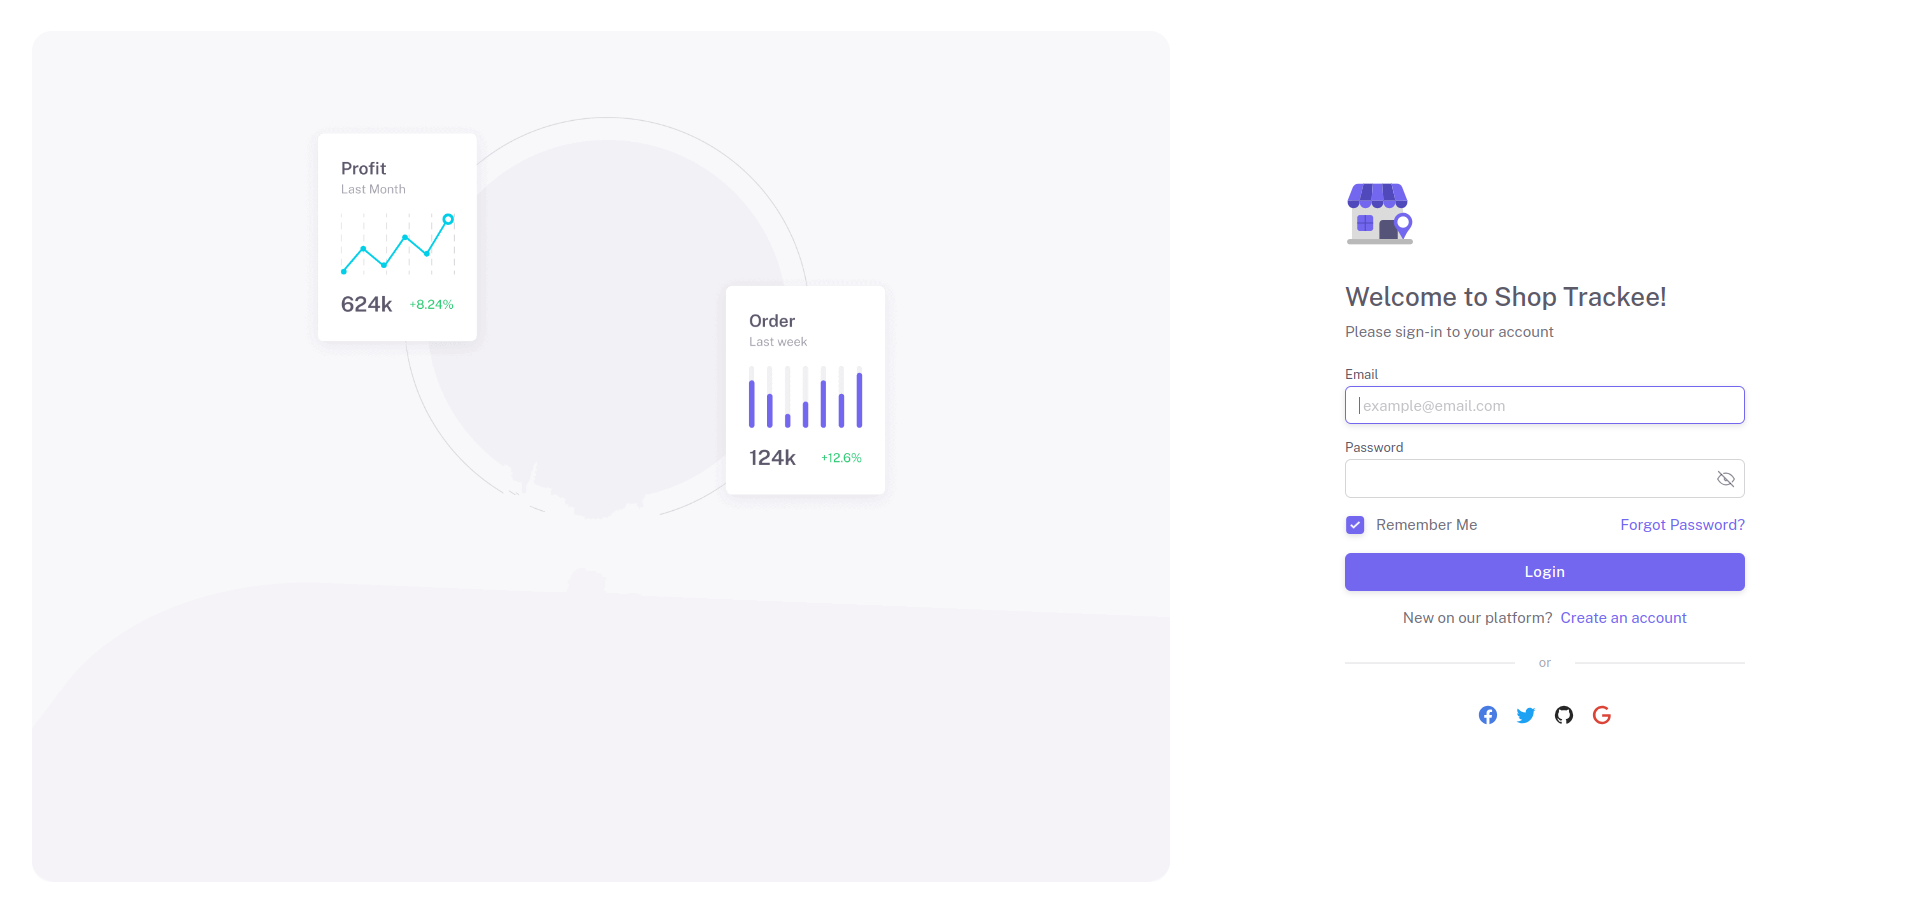
\includegraphics[width=1\textwidth]{login-page}
	\caption{Track My Shop - Login}
\end{figure}

\vspace{2cm}

\begin{figure}[h]
	\subsection{Register\\}
	\centering
	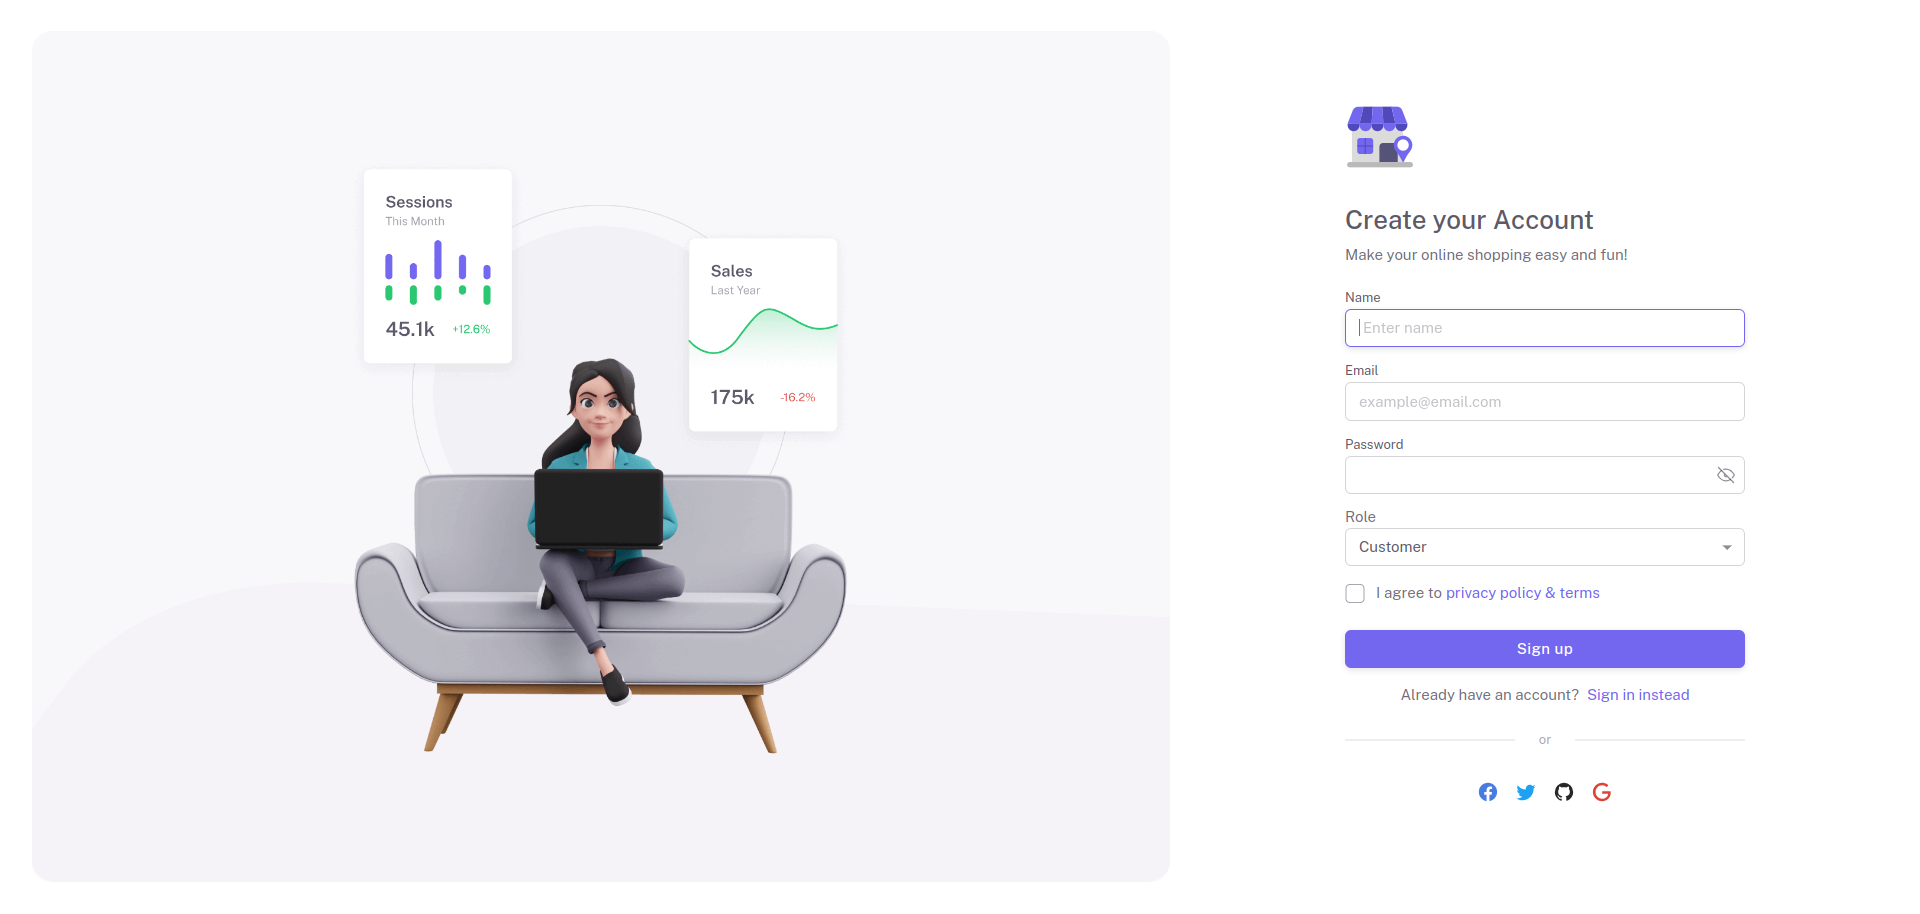
\includegraphics[width=1\textwidth]{signup-page}
	\caption{Track My Shop - Register}
\end{figure}
\newpage

\begin{figure}[h]
	\subsection{Forgot Password\\}
	\centering
	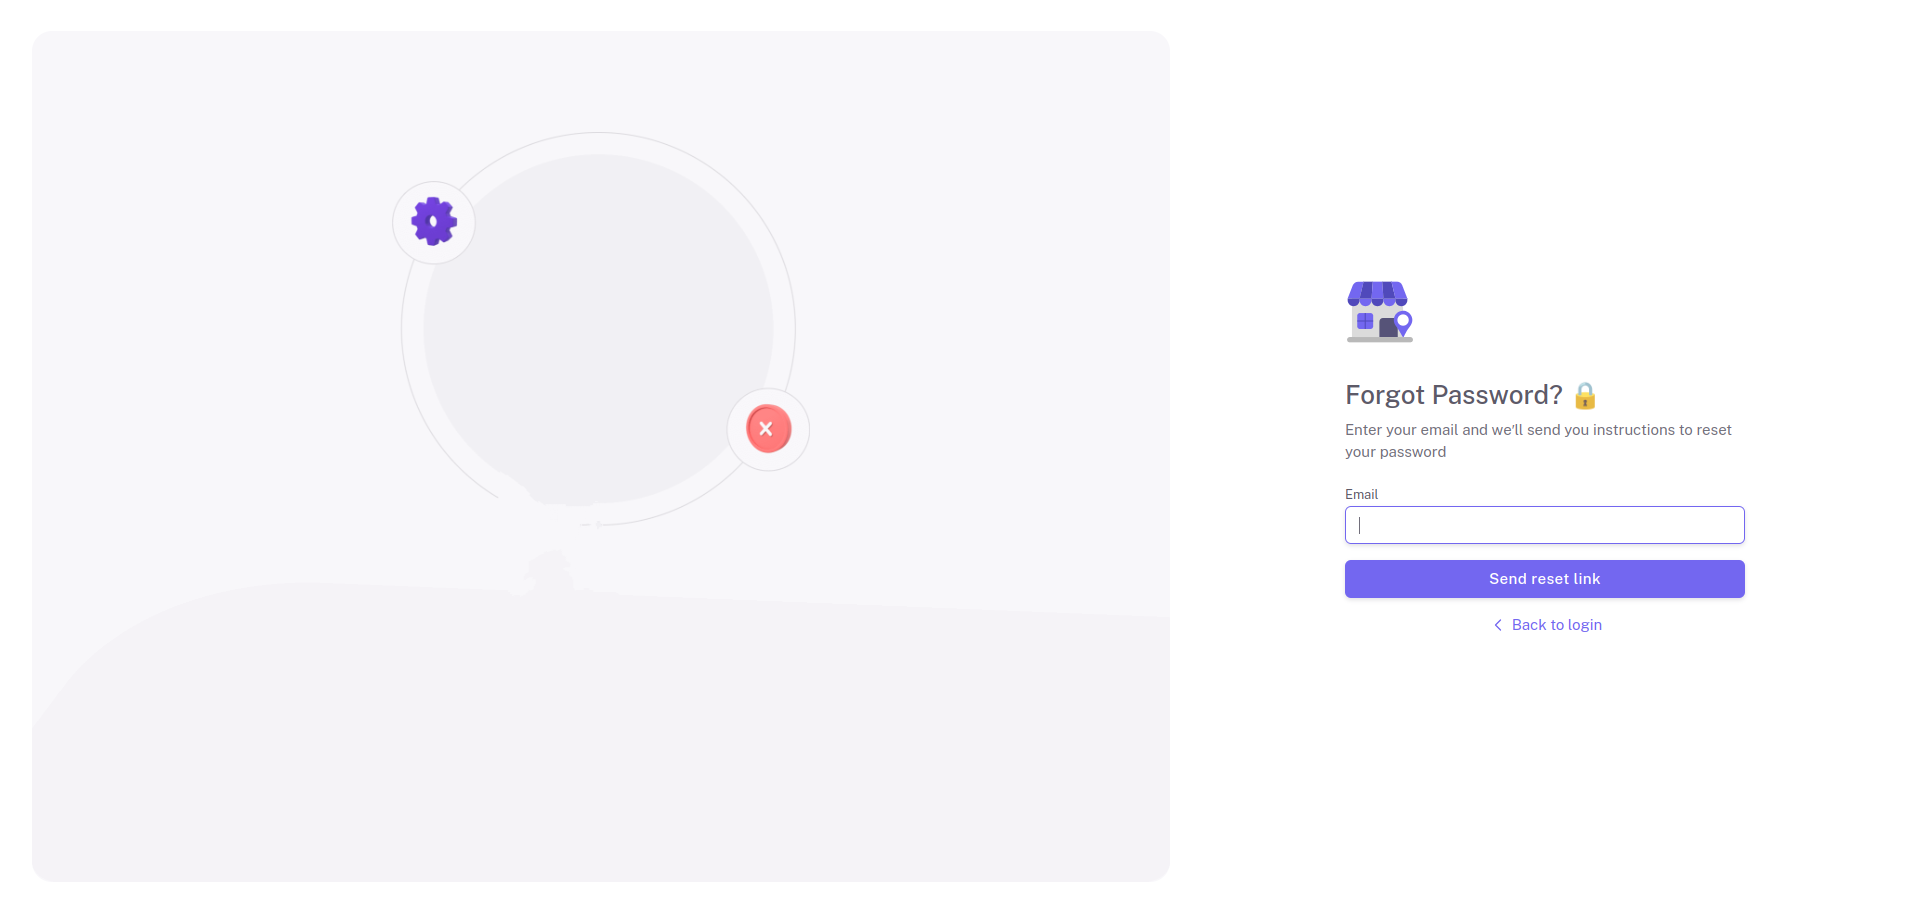
\includegraphics[width=1\textwidth]{forgot-password-page}
	\caption{Track My Shop - Forgot Password}
\end{figure}

\vspace{2cm}

\begin{figure}[h]
	\subsection{Profile\\}
	\centering
	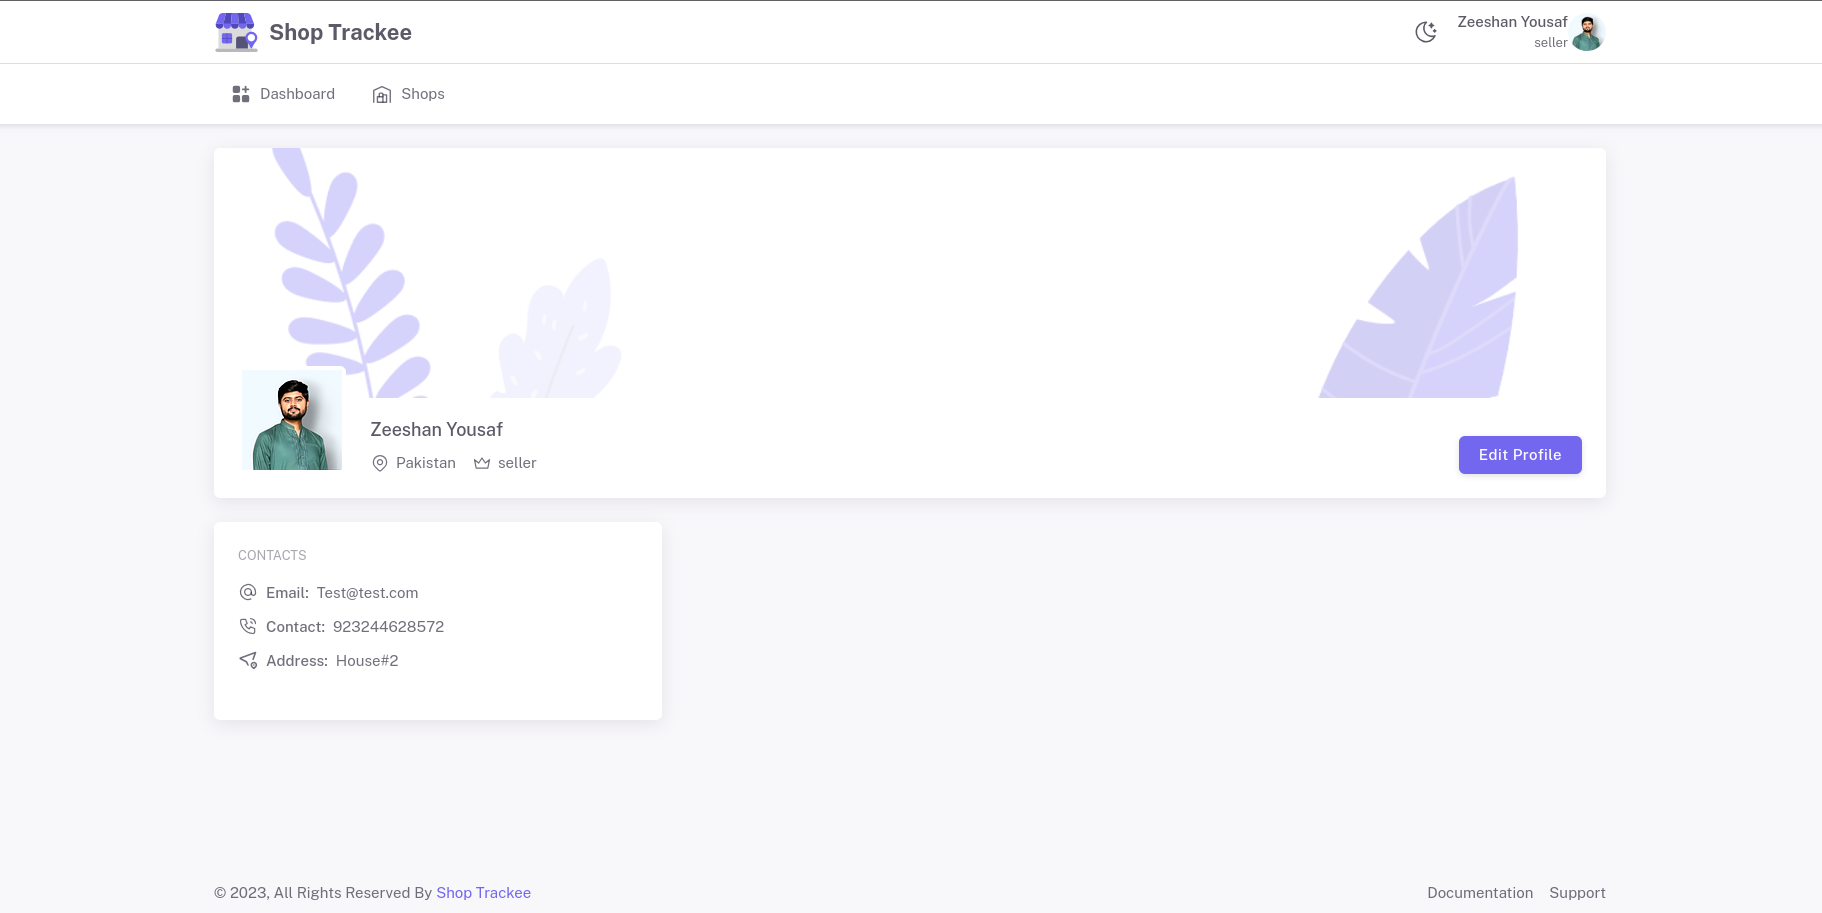
\includegraphics[width=1\textwidth]{seller-profile-page}
	\caption{Track My Shop - Profile}
\end{figure}
\newpage

\begin{figure}[h]
	\subsection{Profile Edit\\}
	\centering
	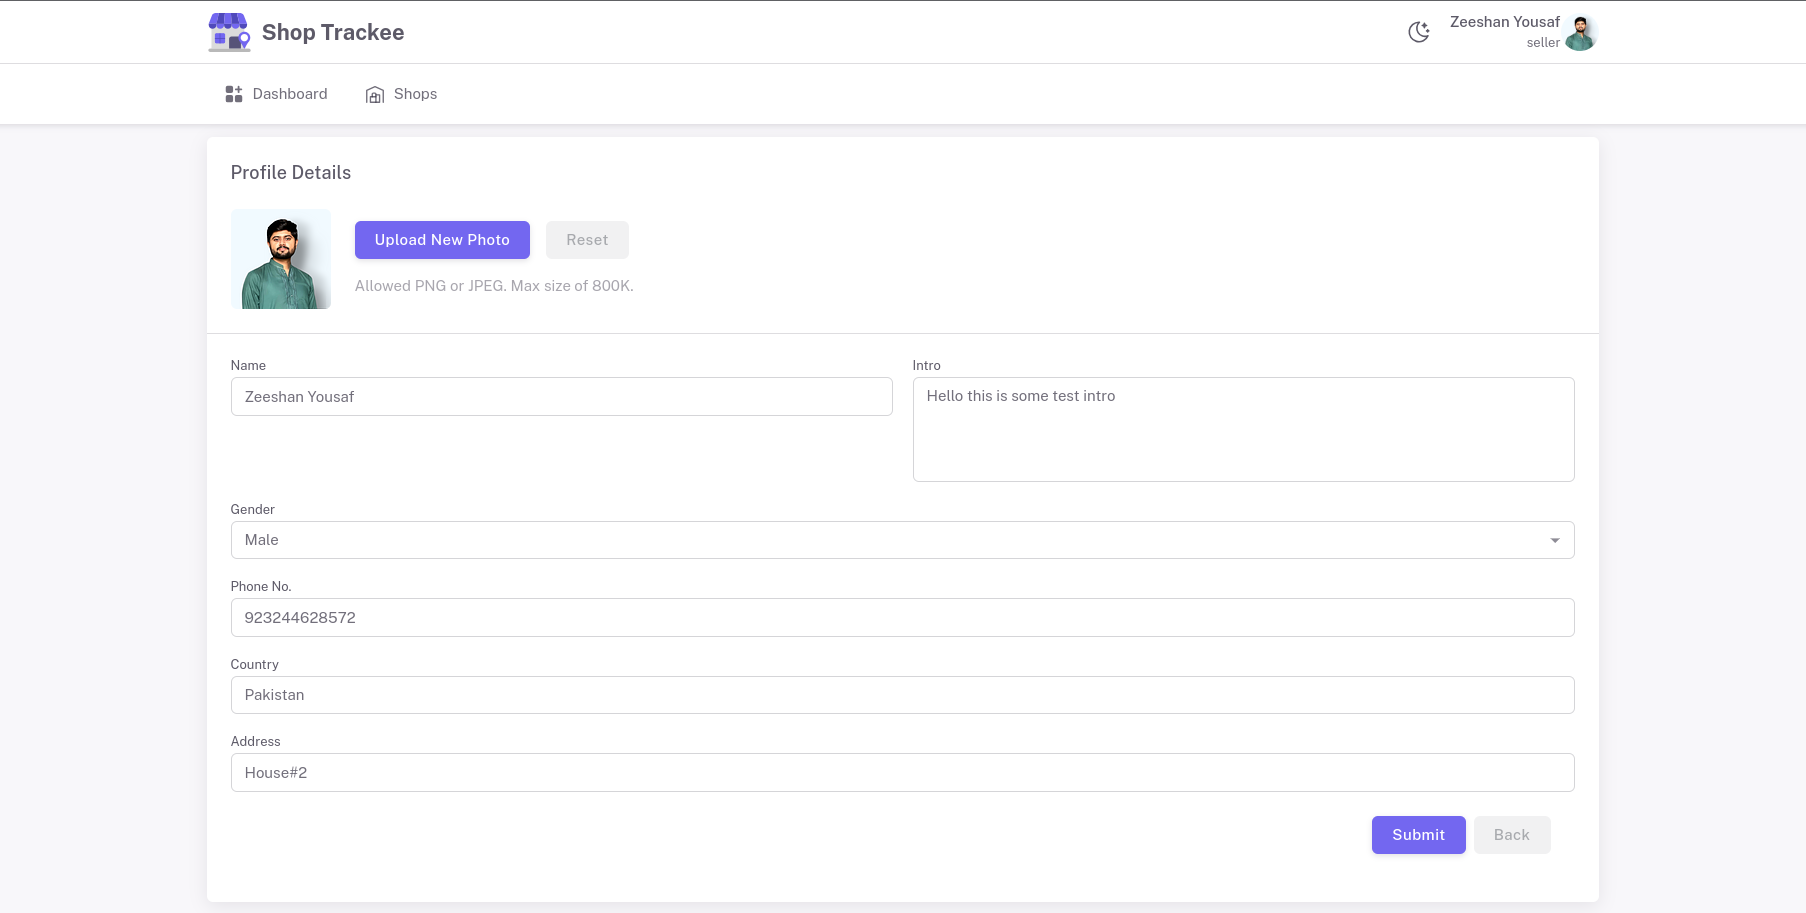
\includegraphics[width=1\textwidth]{profile-edit-page}
	\caption{Track My Shop - Profile Edit}
\end{figure}

\vspace{2cm}

\begin{figure}[h]
	\subsection{Seller Dashboard\\}
	\centering
	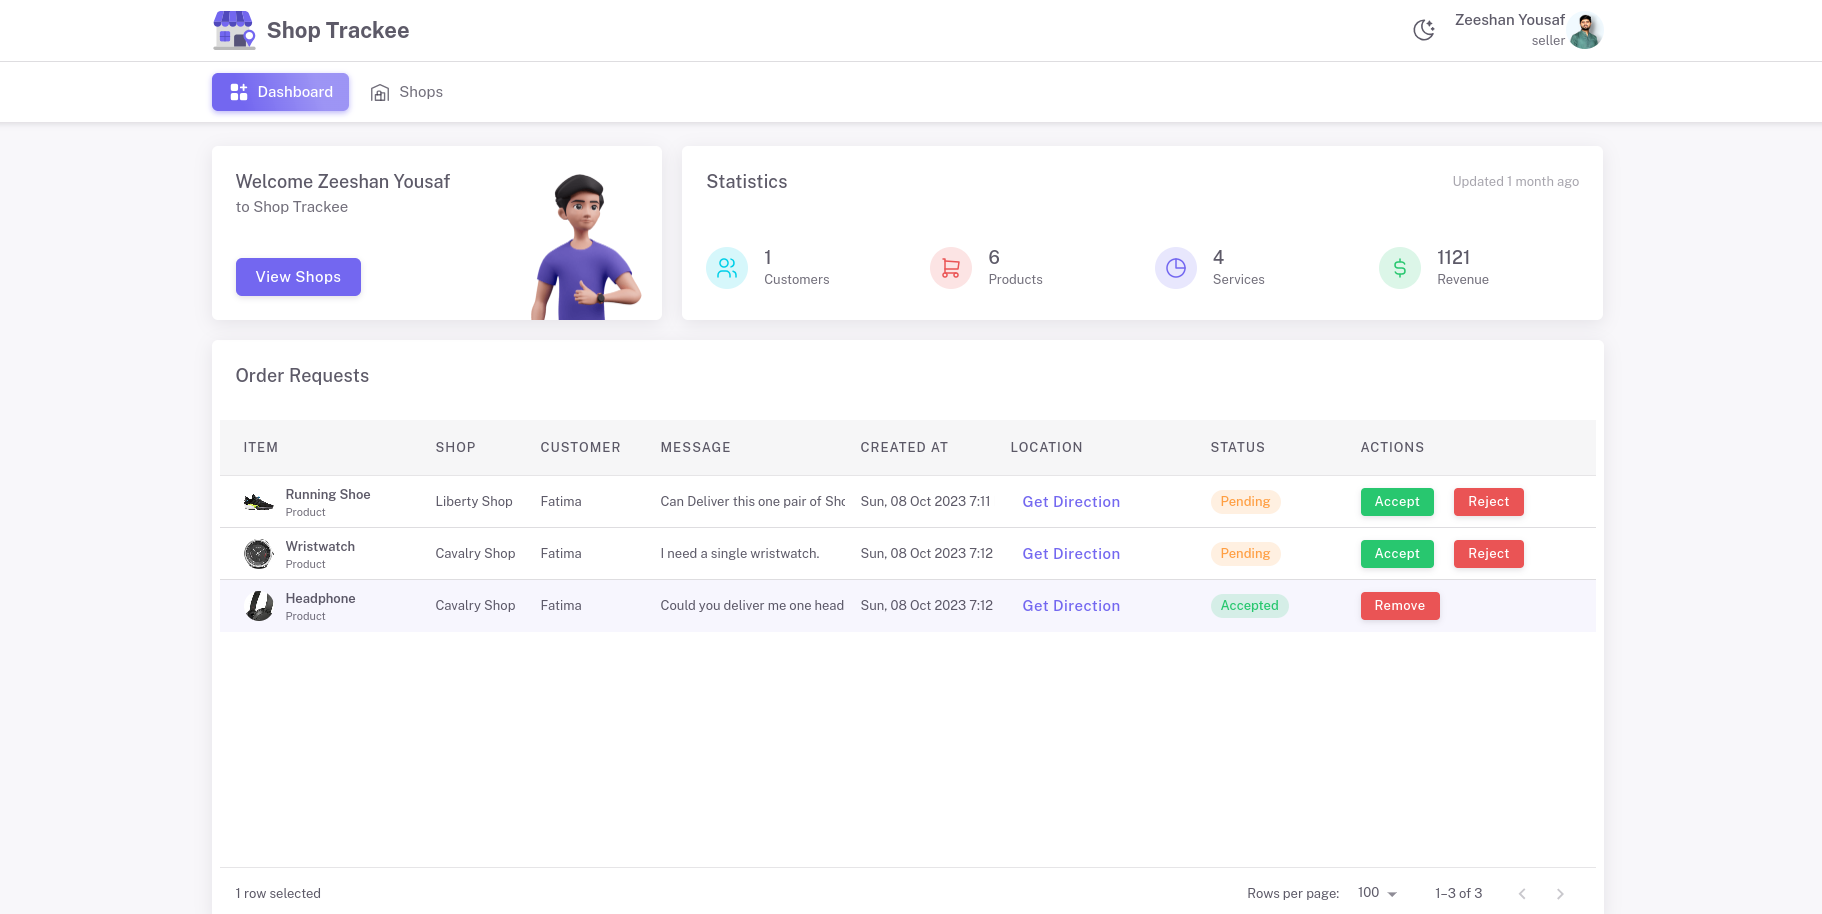
\includegraphics[width=1\textwidth]{seller-dashboard-page}
	\caption{Track My Shop - Seller Dashboard}
\end{figure}
\newpage

\begin{figure}[h]
	\subsection{Seller Shops\\}
	\centering
	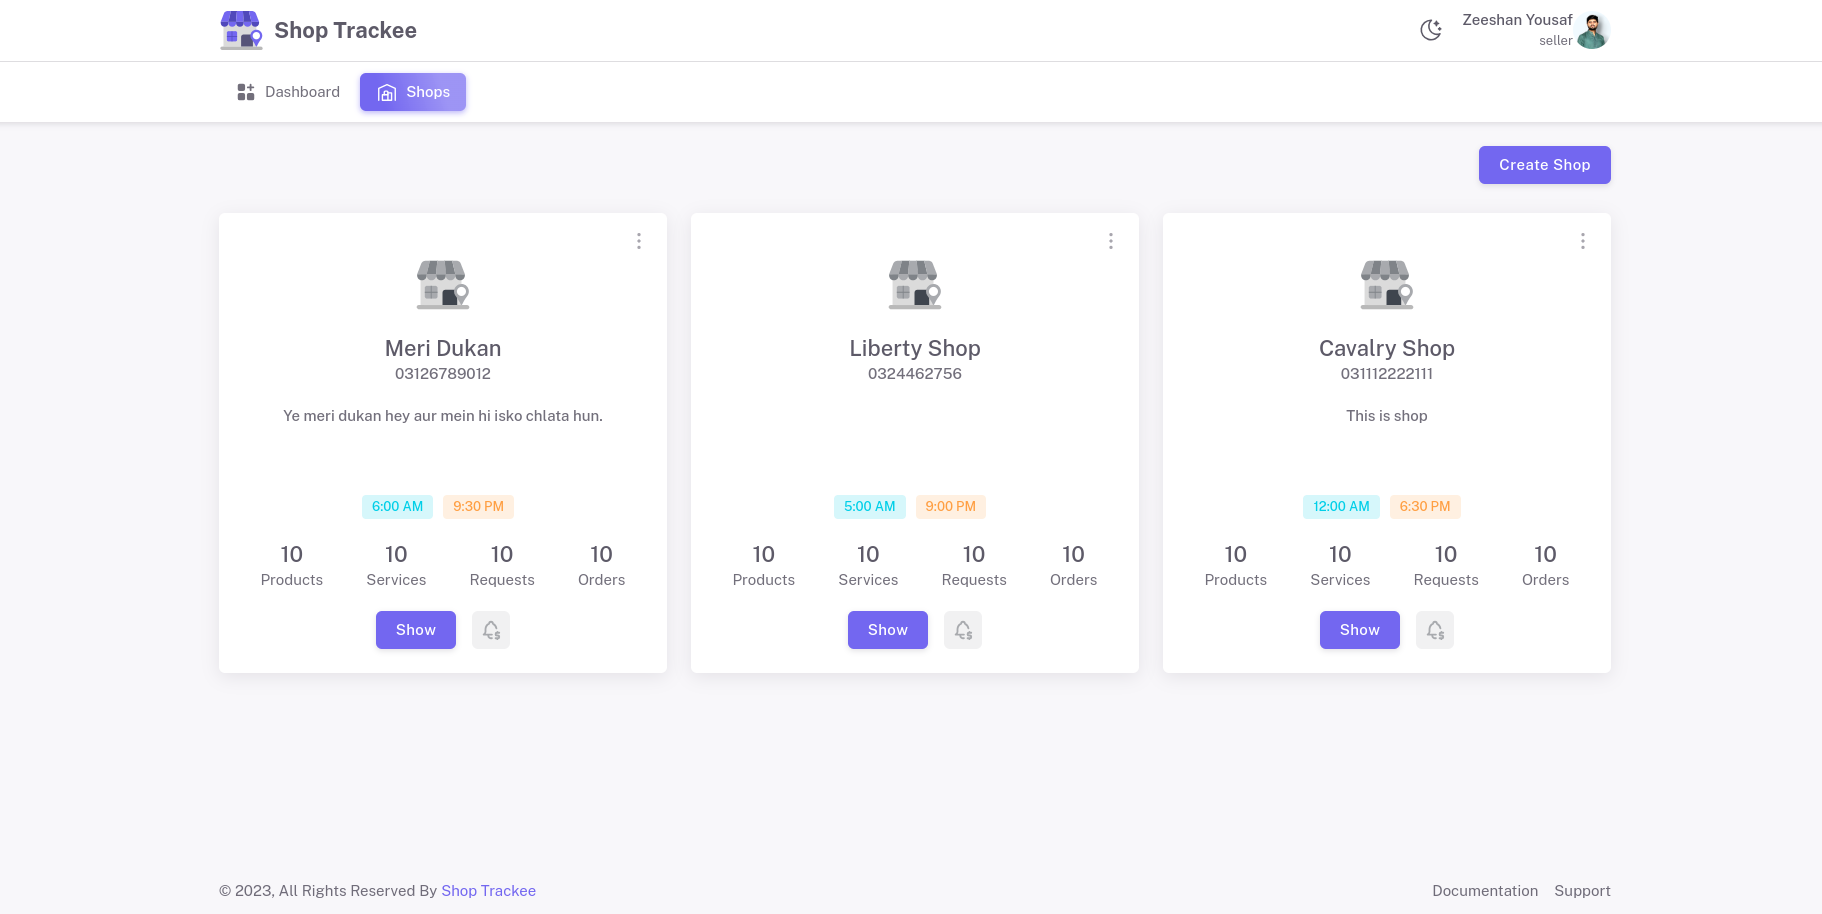
\includegraphics[width=1\textwidth]{seller-shops-page}
	\caption{Track My Shop - Seller Shops}
\end{figure}

\vspace{2cm}

\begin{figure}[h]
	\subsection{Seller Create Shop \\}
	\centering
	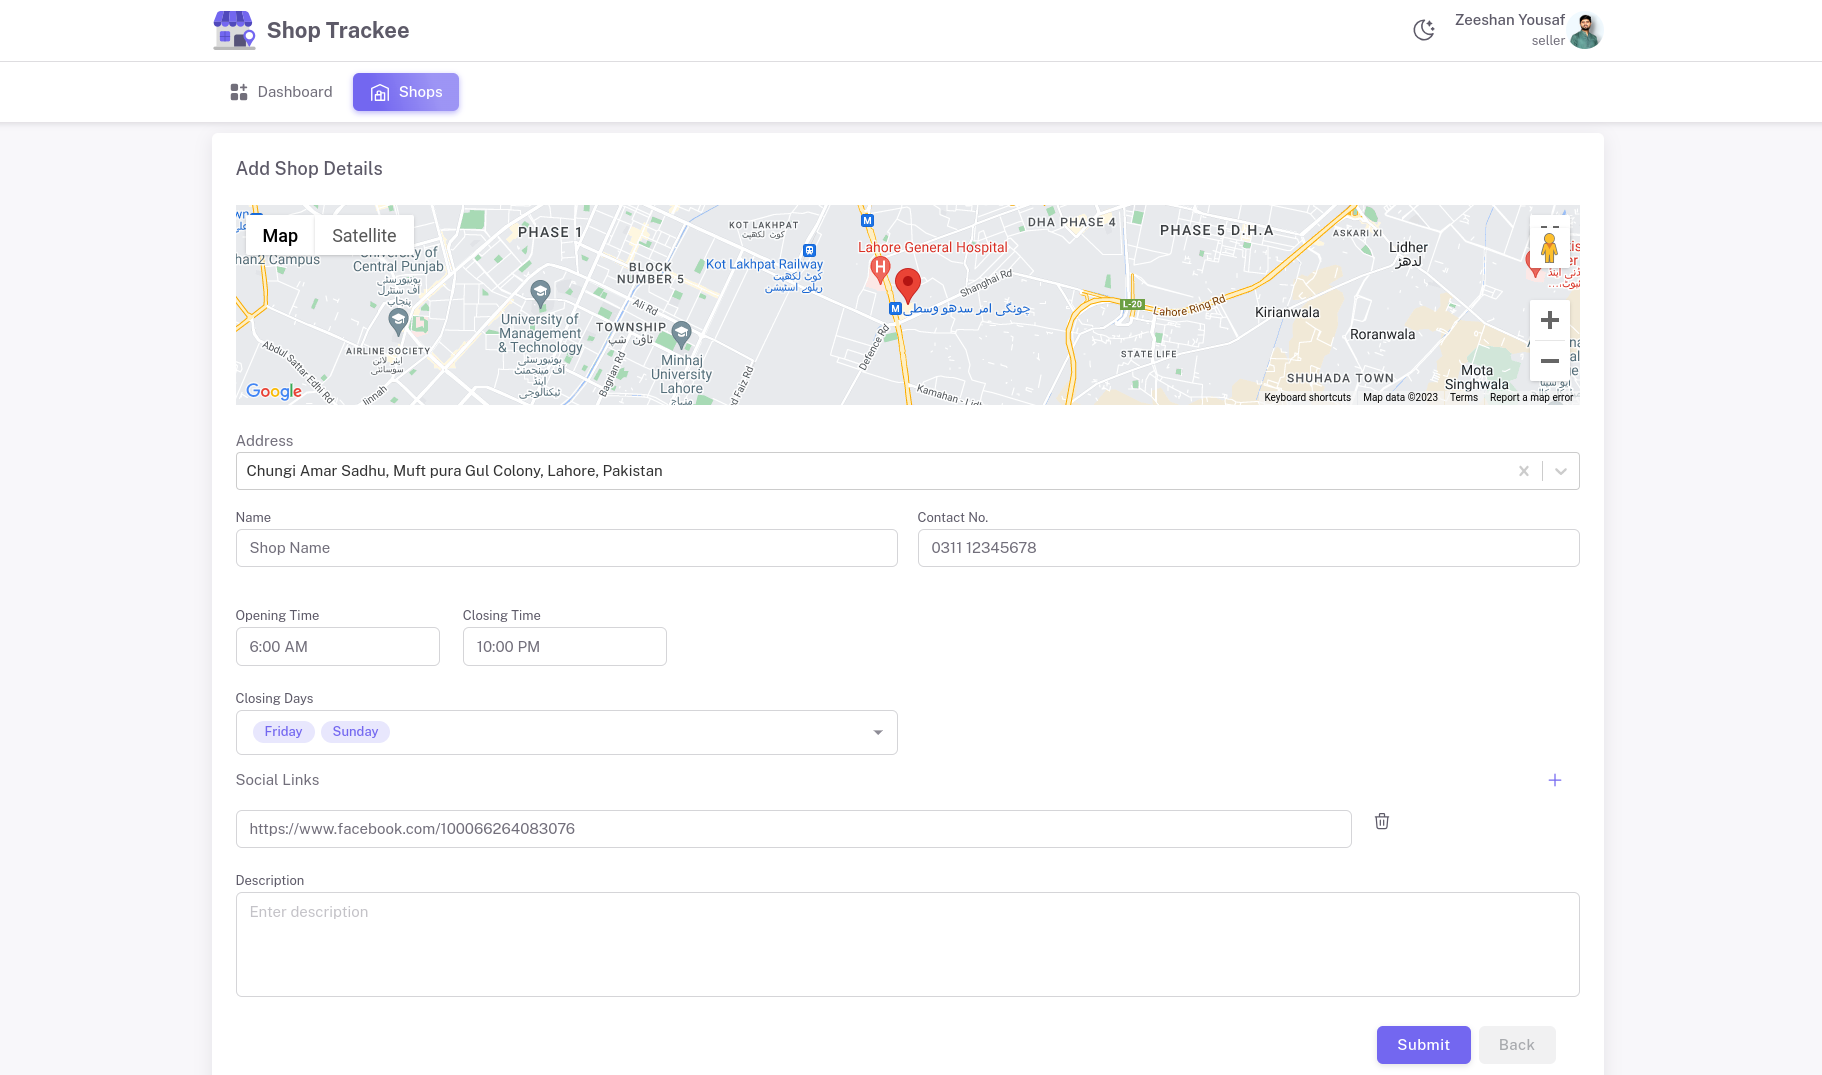
\includegraphics[width=0.9\textwidth]{seller-shop-create-page}
	\caption{Track My Shop - Create Shop}
\end{figure}
\newpage

\begin{figure}[h]
	\subsection{Seller Add Product }
	\centering
	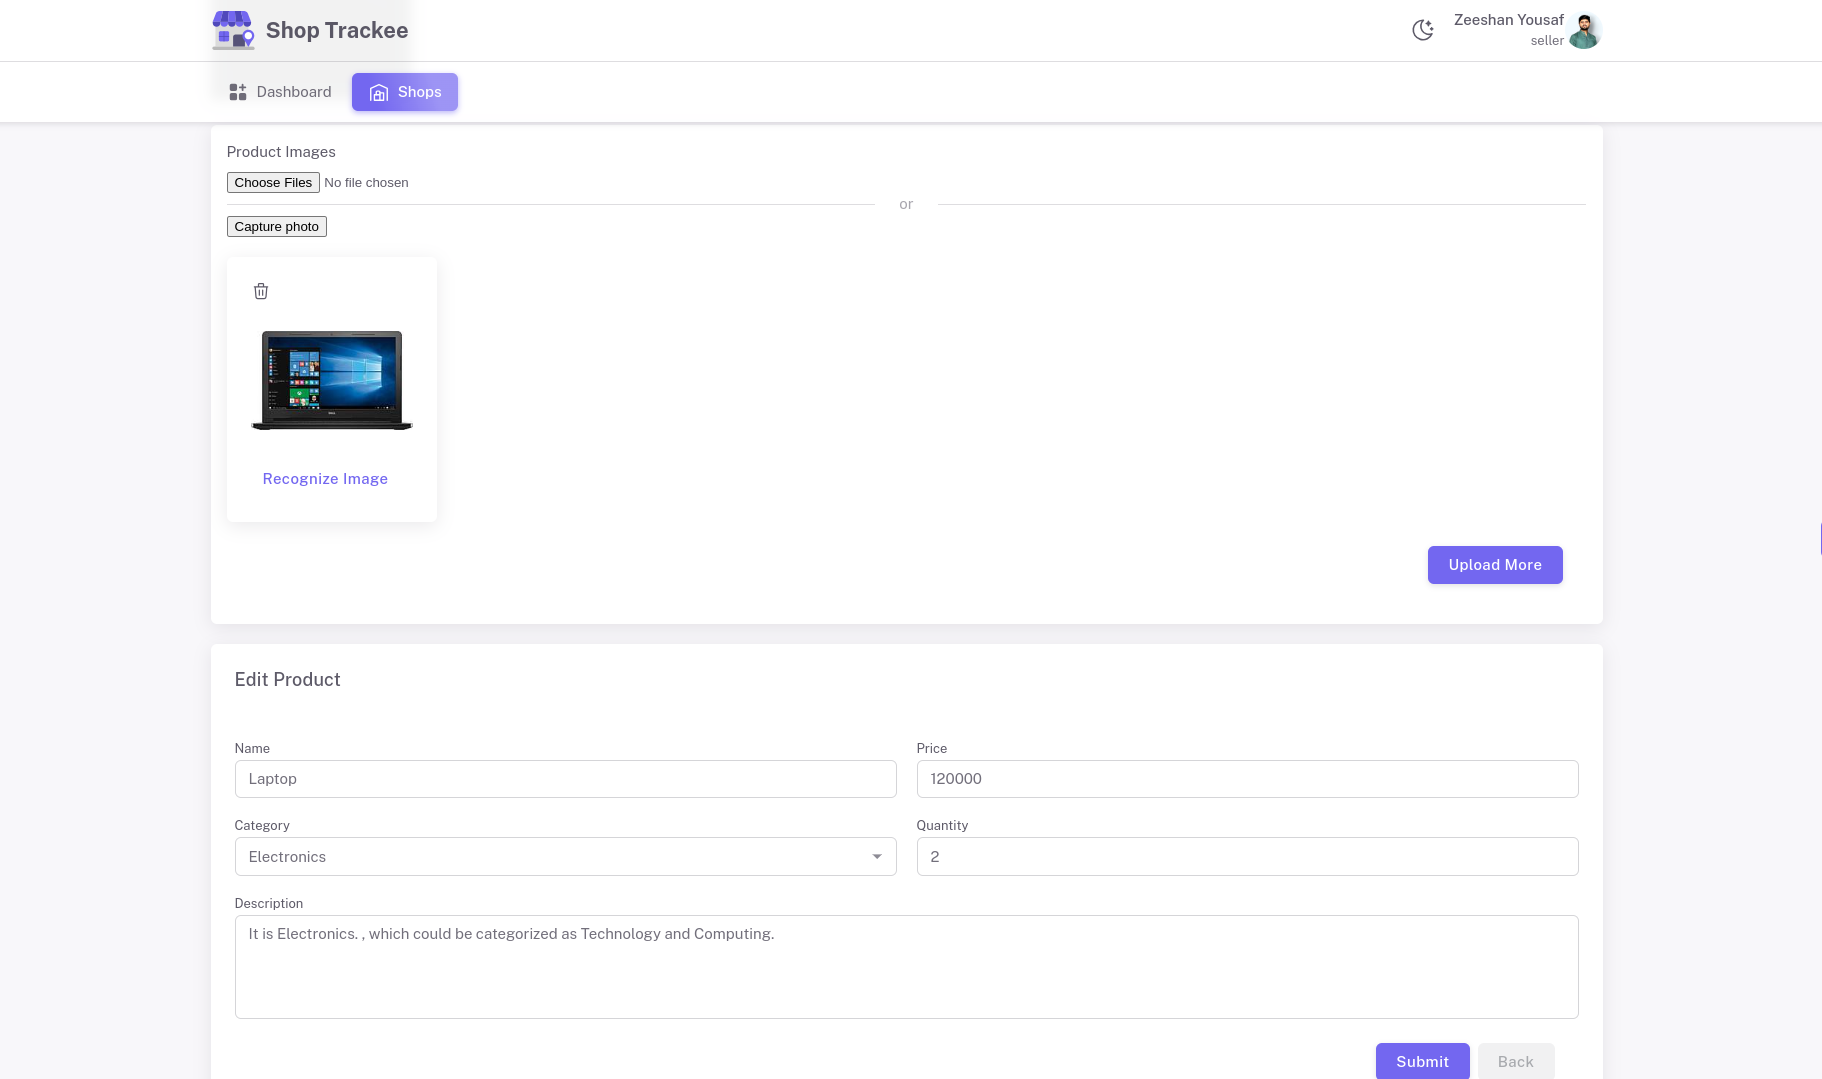
\includegraphics[width=1\textwidth]{product-form-page}
	\caption{Track My Shop - Add Product}
\end{figure}
\vspace{0.5cm}
\begin{figure}[h]
	\subsection{Seller Add Service \\}
	\centering
	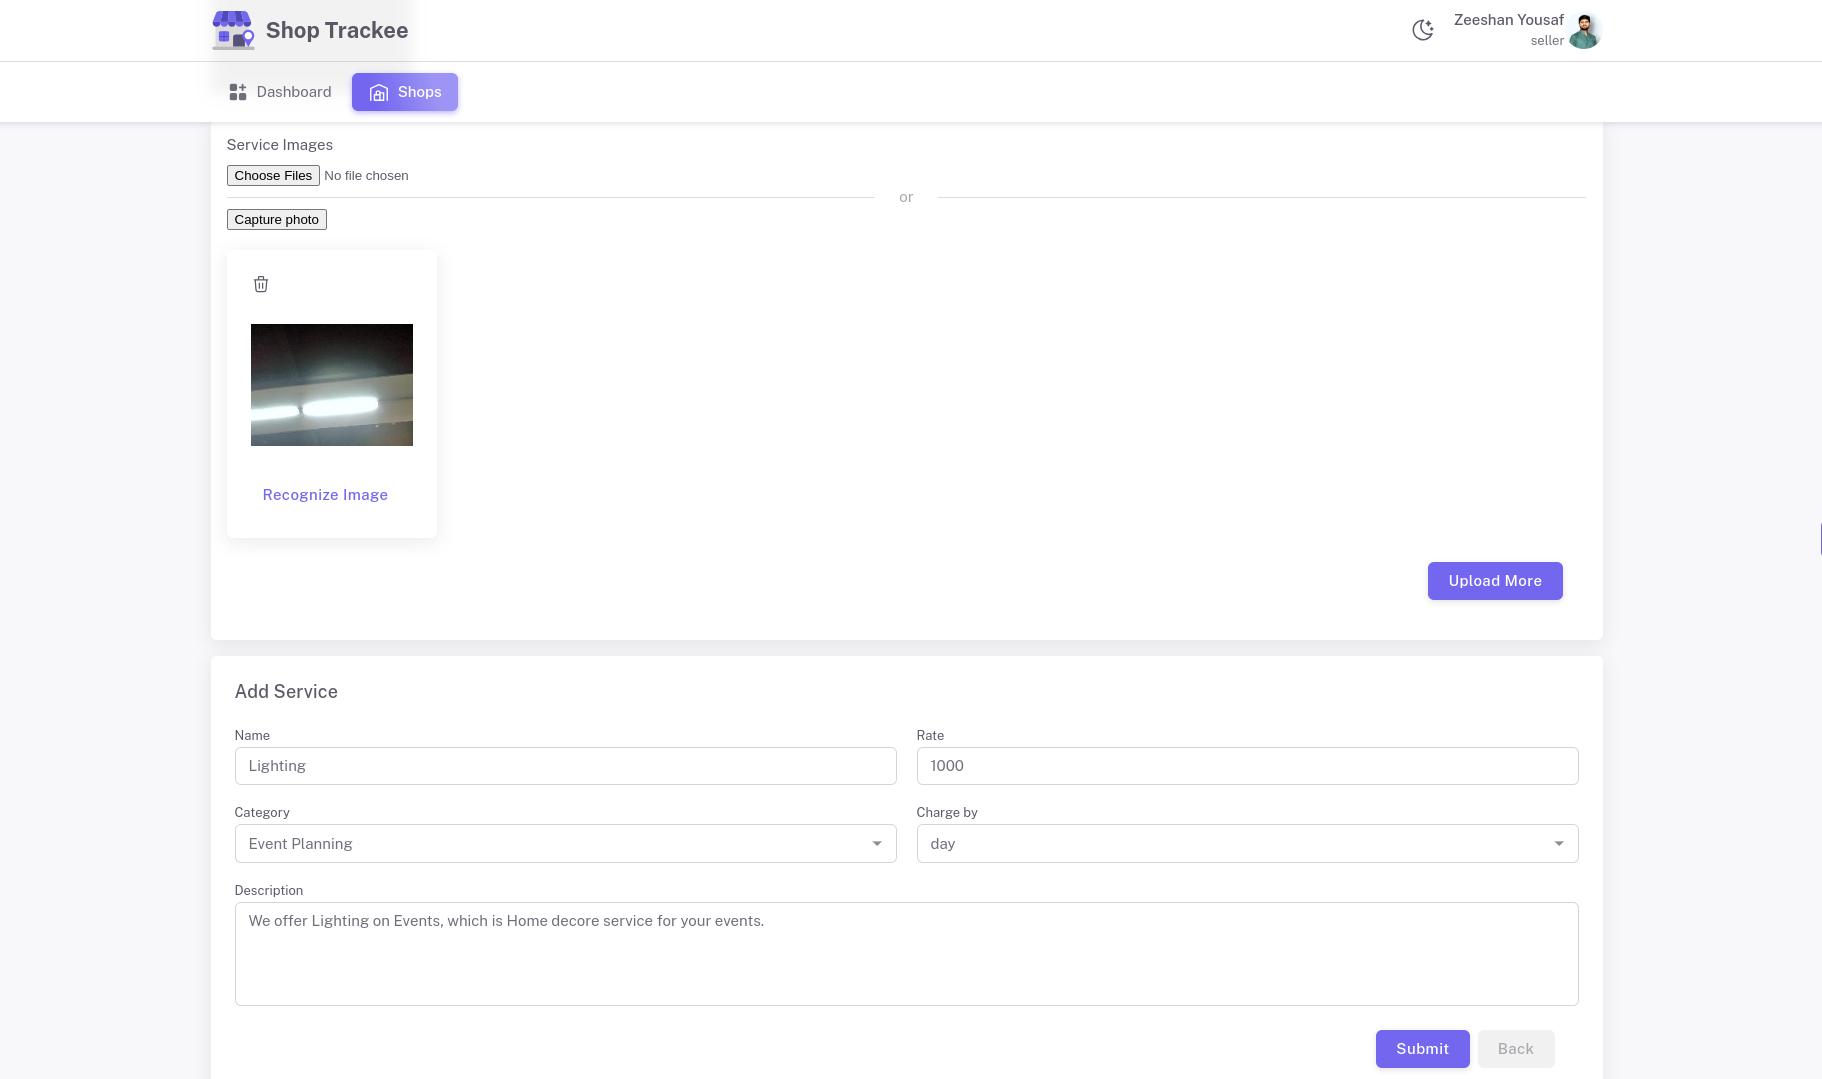
\includegraphics[width=0.9\textwidth]{service-form-page}
	\caption{Track My Shop - Add Service}
\end{figure}
\newpage

\begin{figure}[h]
	\subsection{Seller Products and Services Listing}
	\centering
	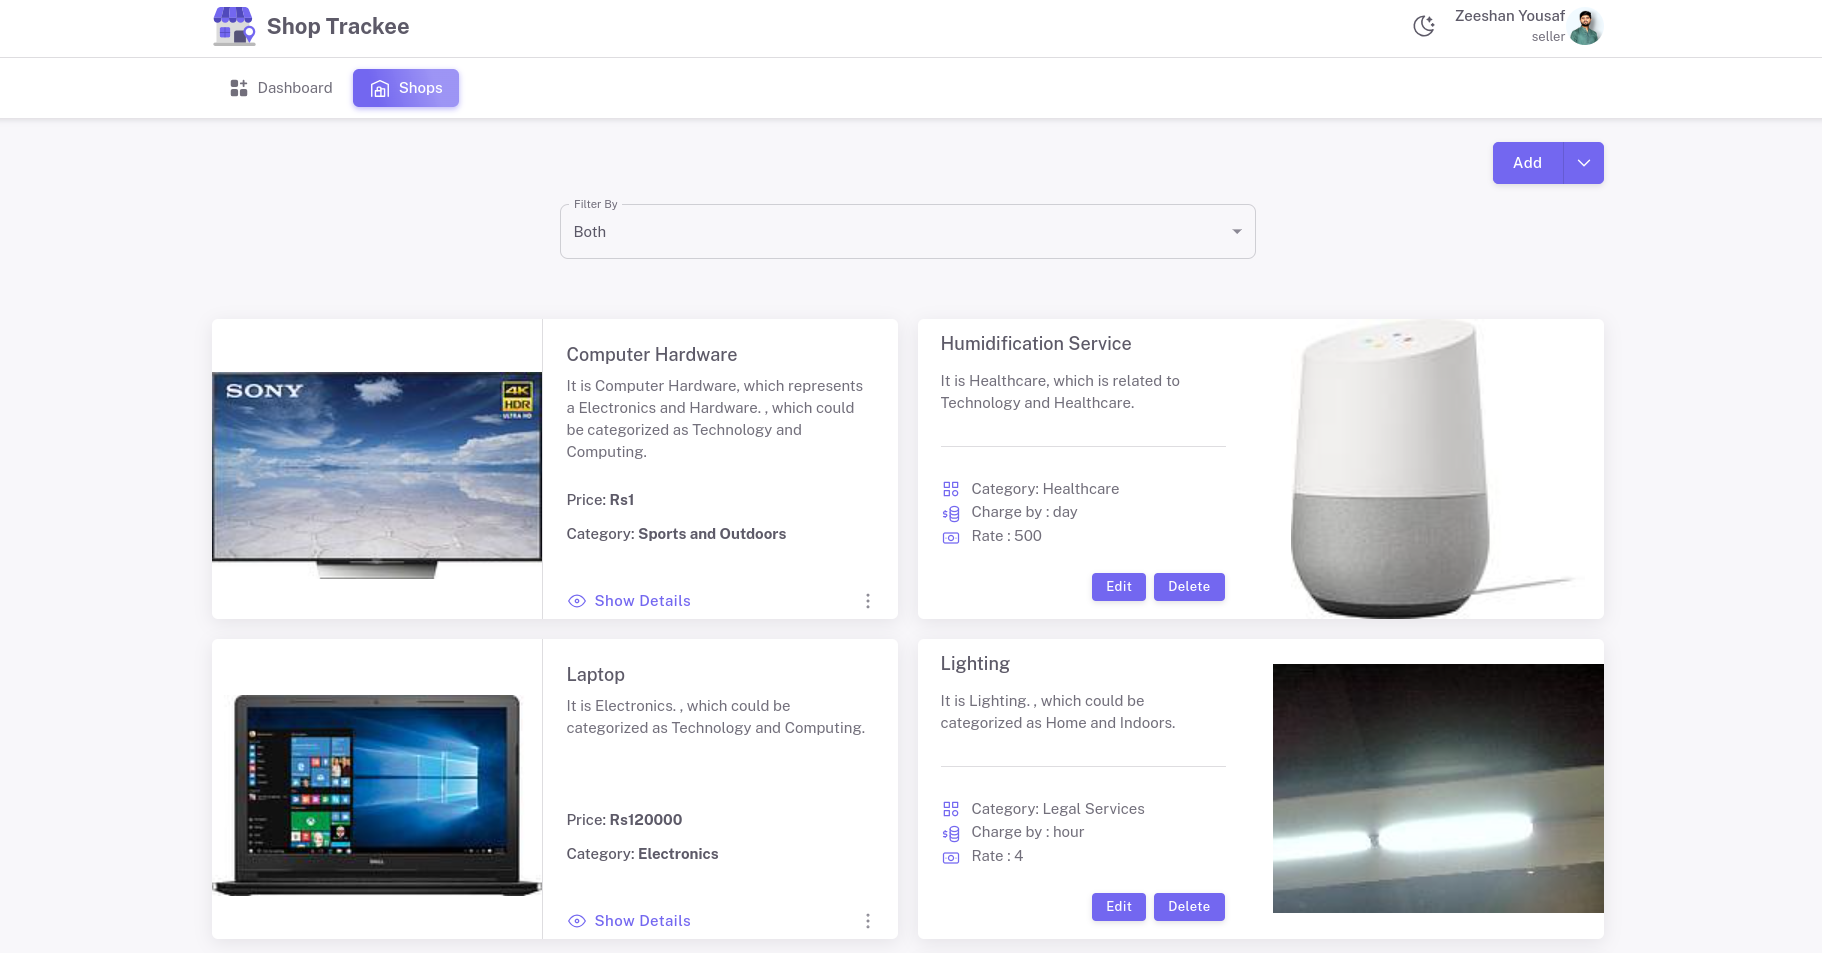
\includegraphics[width=1\textwidth]{products-services-page}
	\caption{Track My Shop - Products and Services Listing}
\end{figure}


\begin{figure}[h]
	\subsection{Customer Home \\}
	\centering
	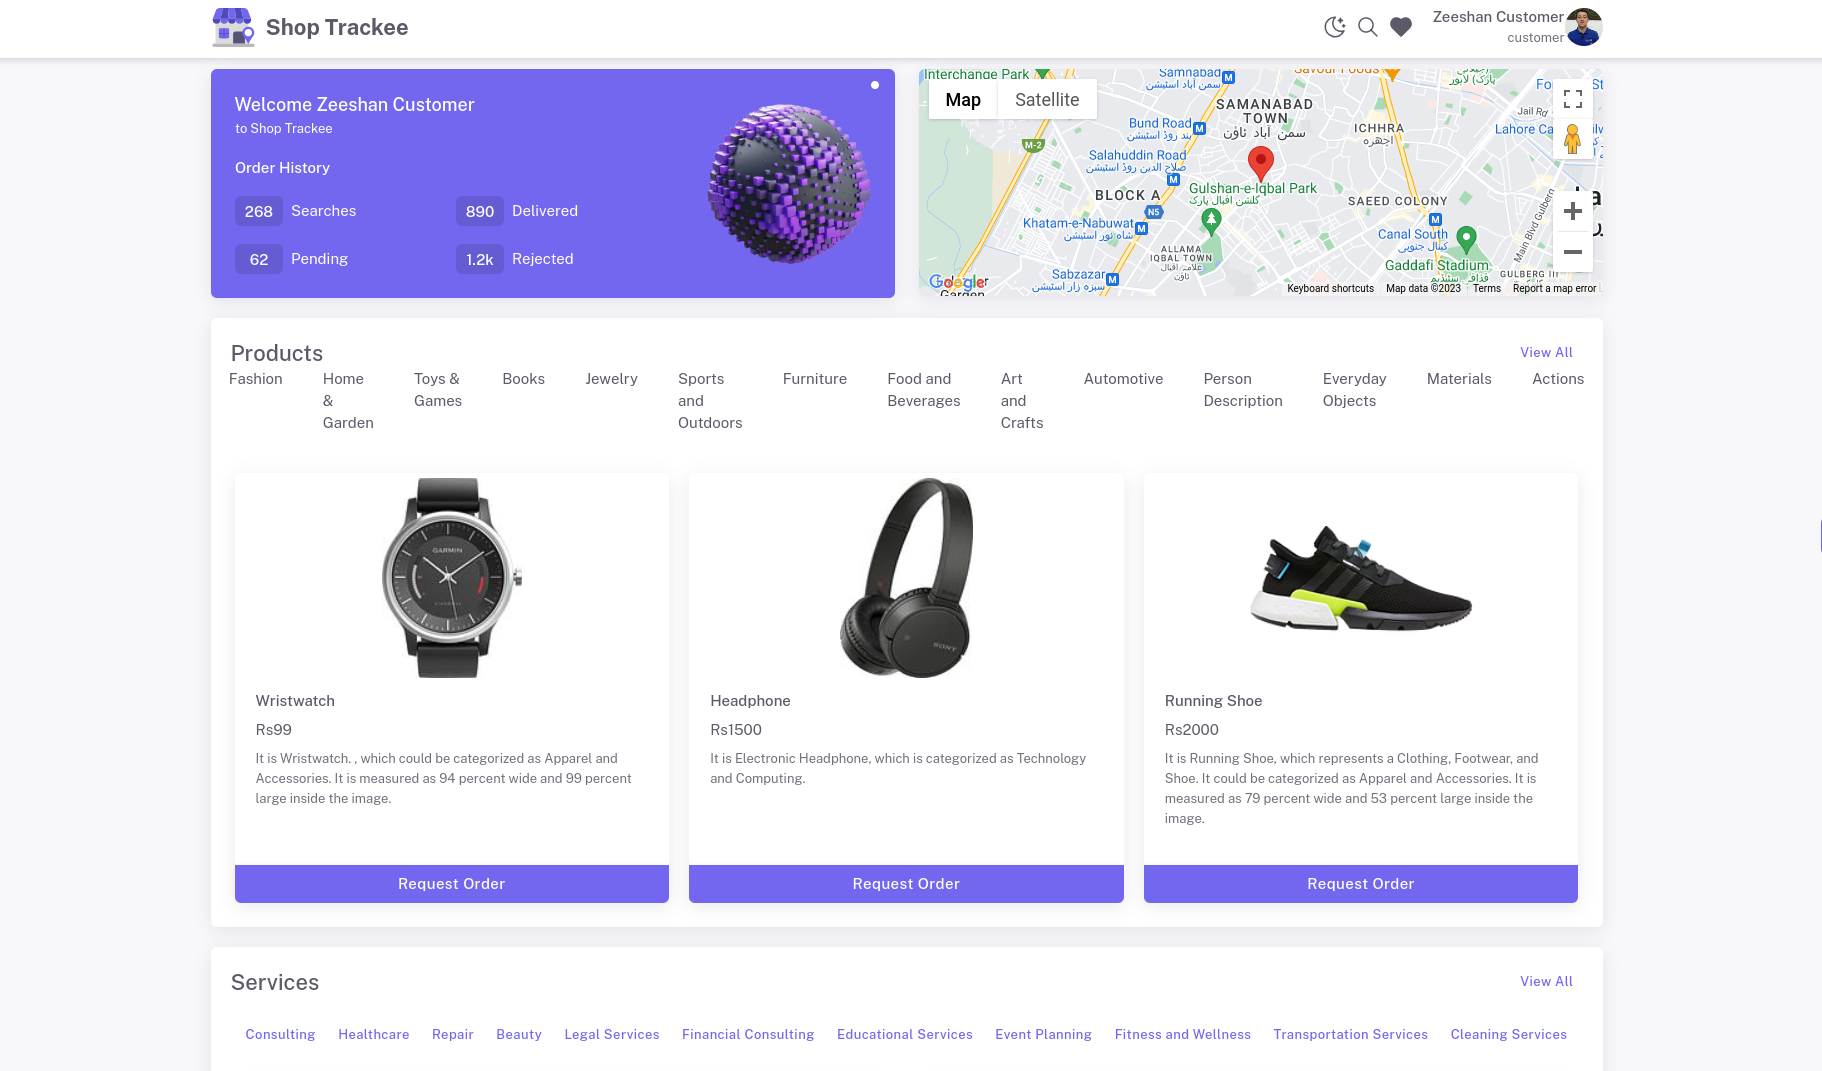
\includegraphics[width=1\textwidth]{customer-home-page}
	\caption{Track My Shop - Customer Home}
\end{figure}
\newpage

\begin{figure}[h]
	\subsection{Customer Searching Around \\}
	\centering
	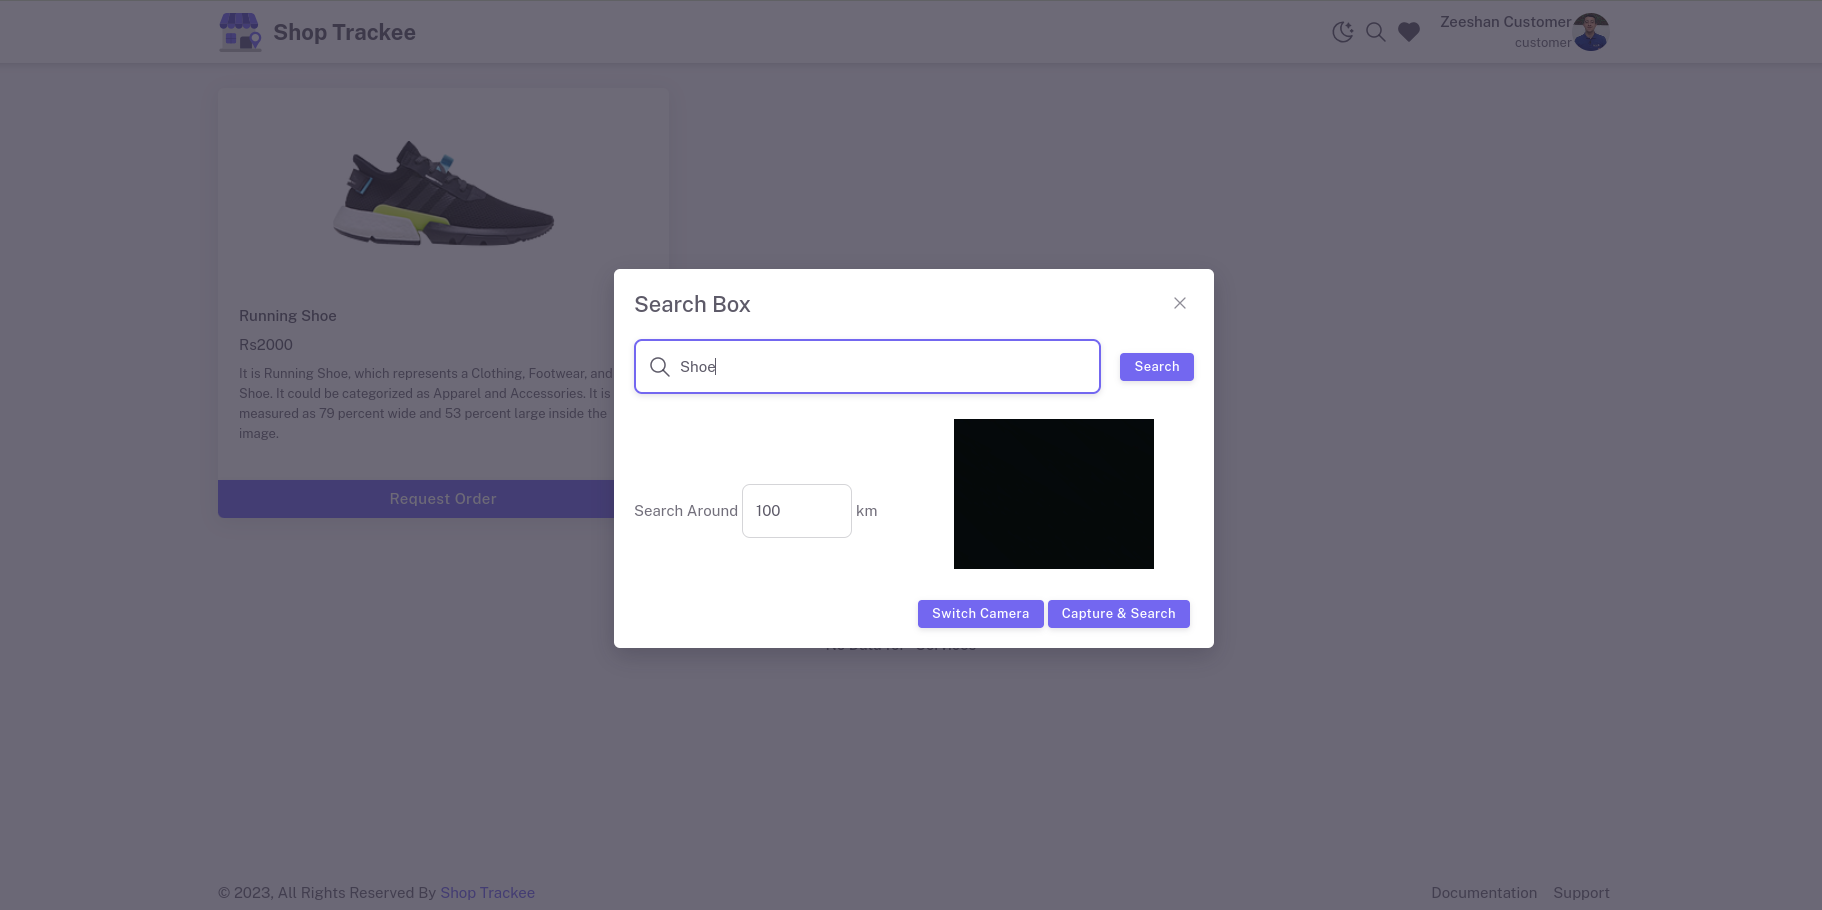
\includegraphics[width=1\textwidth]{searching-page}
	\caption{Track My Shop - Customer Searching Around}
\end{figure}

\vspace{1cm}

\begin{figure}[h]
	\subsection{Customer Requesting Order \\}
	\centering
	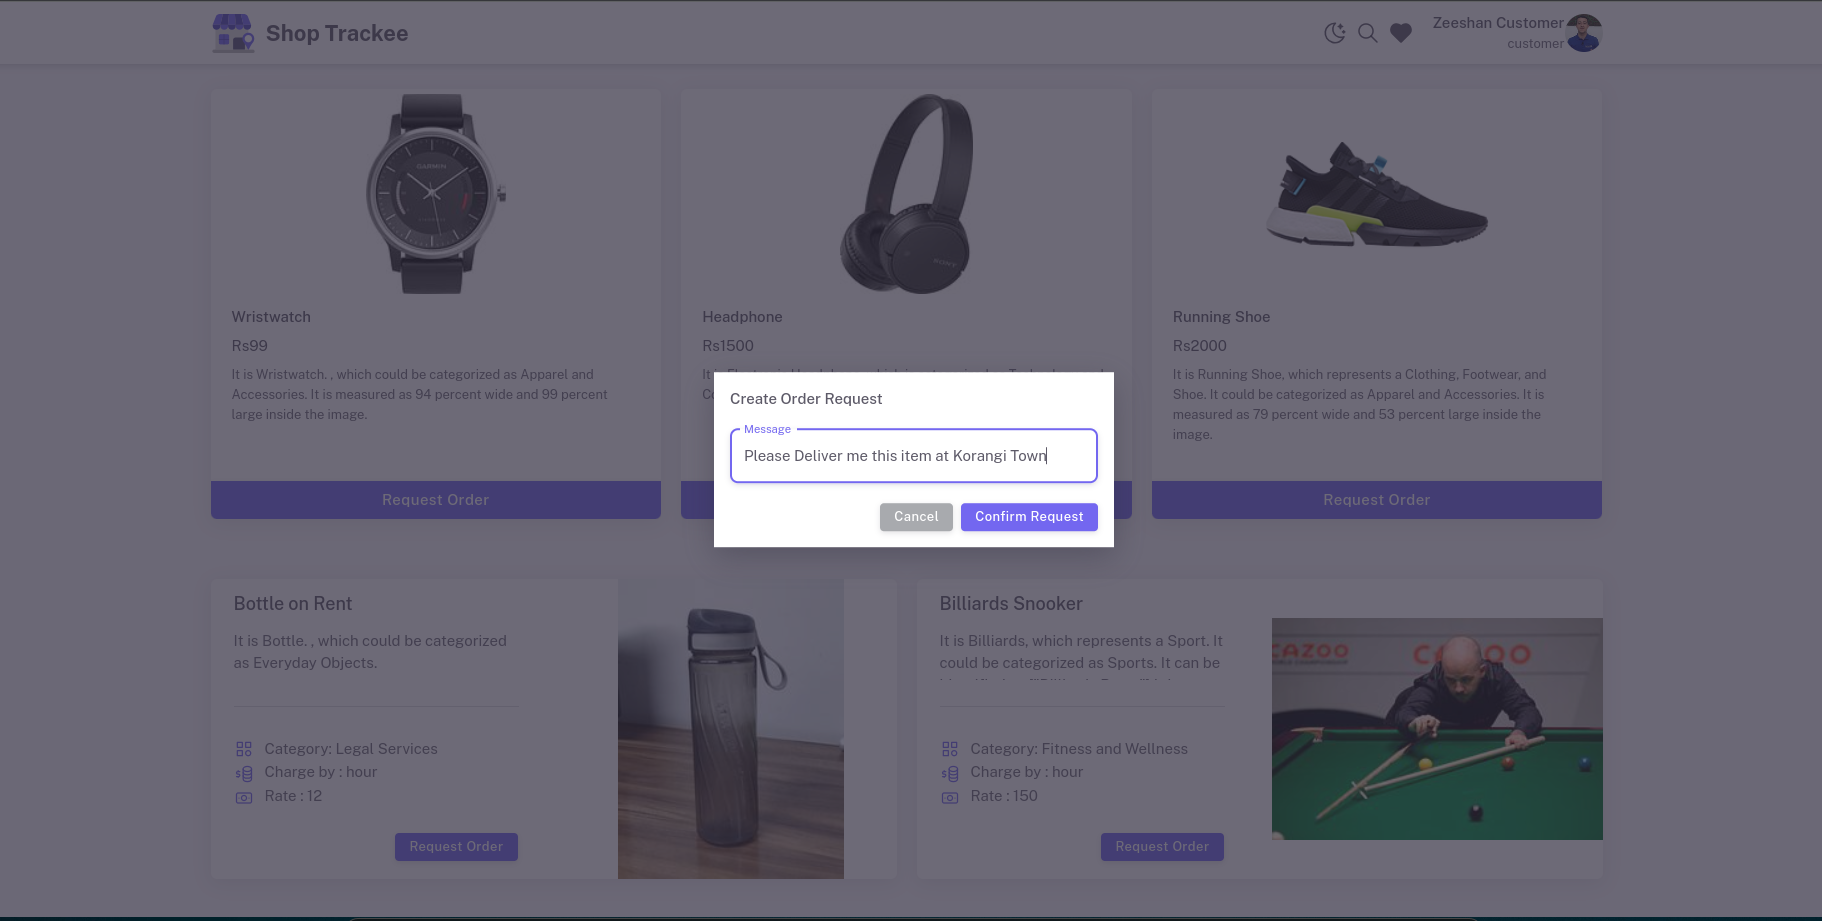
\includegraphics[width=1\textwidth]{requesting-order-page}
	\caption{Track My Shop - Customer Requesting Order}
\end{figure}
\newpage

\begin{figure}[h]
	\subsection{Customer Order Requests History \\}
	\centering
	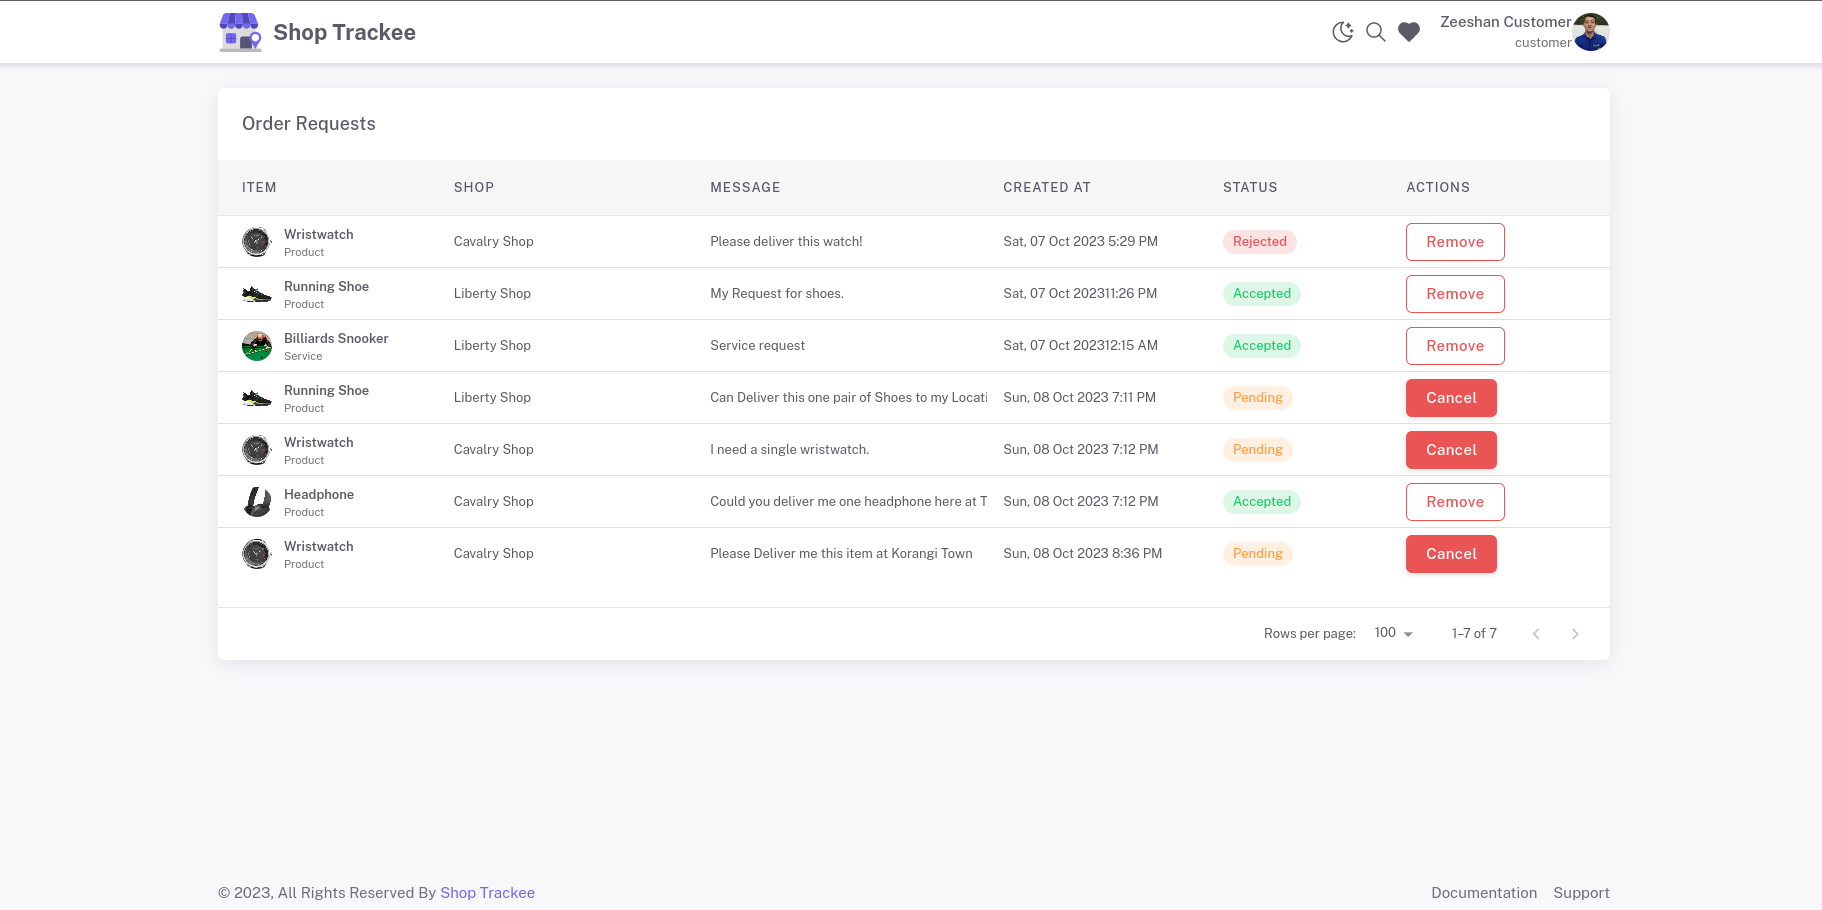
\includegraphics[width=1\textwidth]{customer-order-requests-page}
	\caption{Track My Shop - Customer Order Requests History}
\end{figure}

\begin{figure}[h]
	\subsection{Customer Favorites \\}
	\centering
	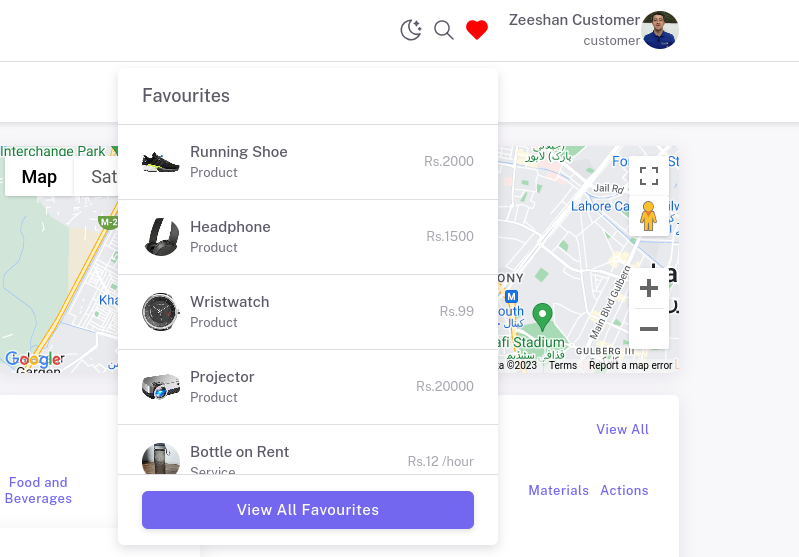
\includegraphics[width=0.8\textwidth]{customer-home-favorites-page}
	\caption{Track My Shop - Customer Favorites}
\end{figure}
\pagebreak
\begin{figure}[h]
	\subsection{Customer All Favorites}
	\centering
	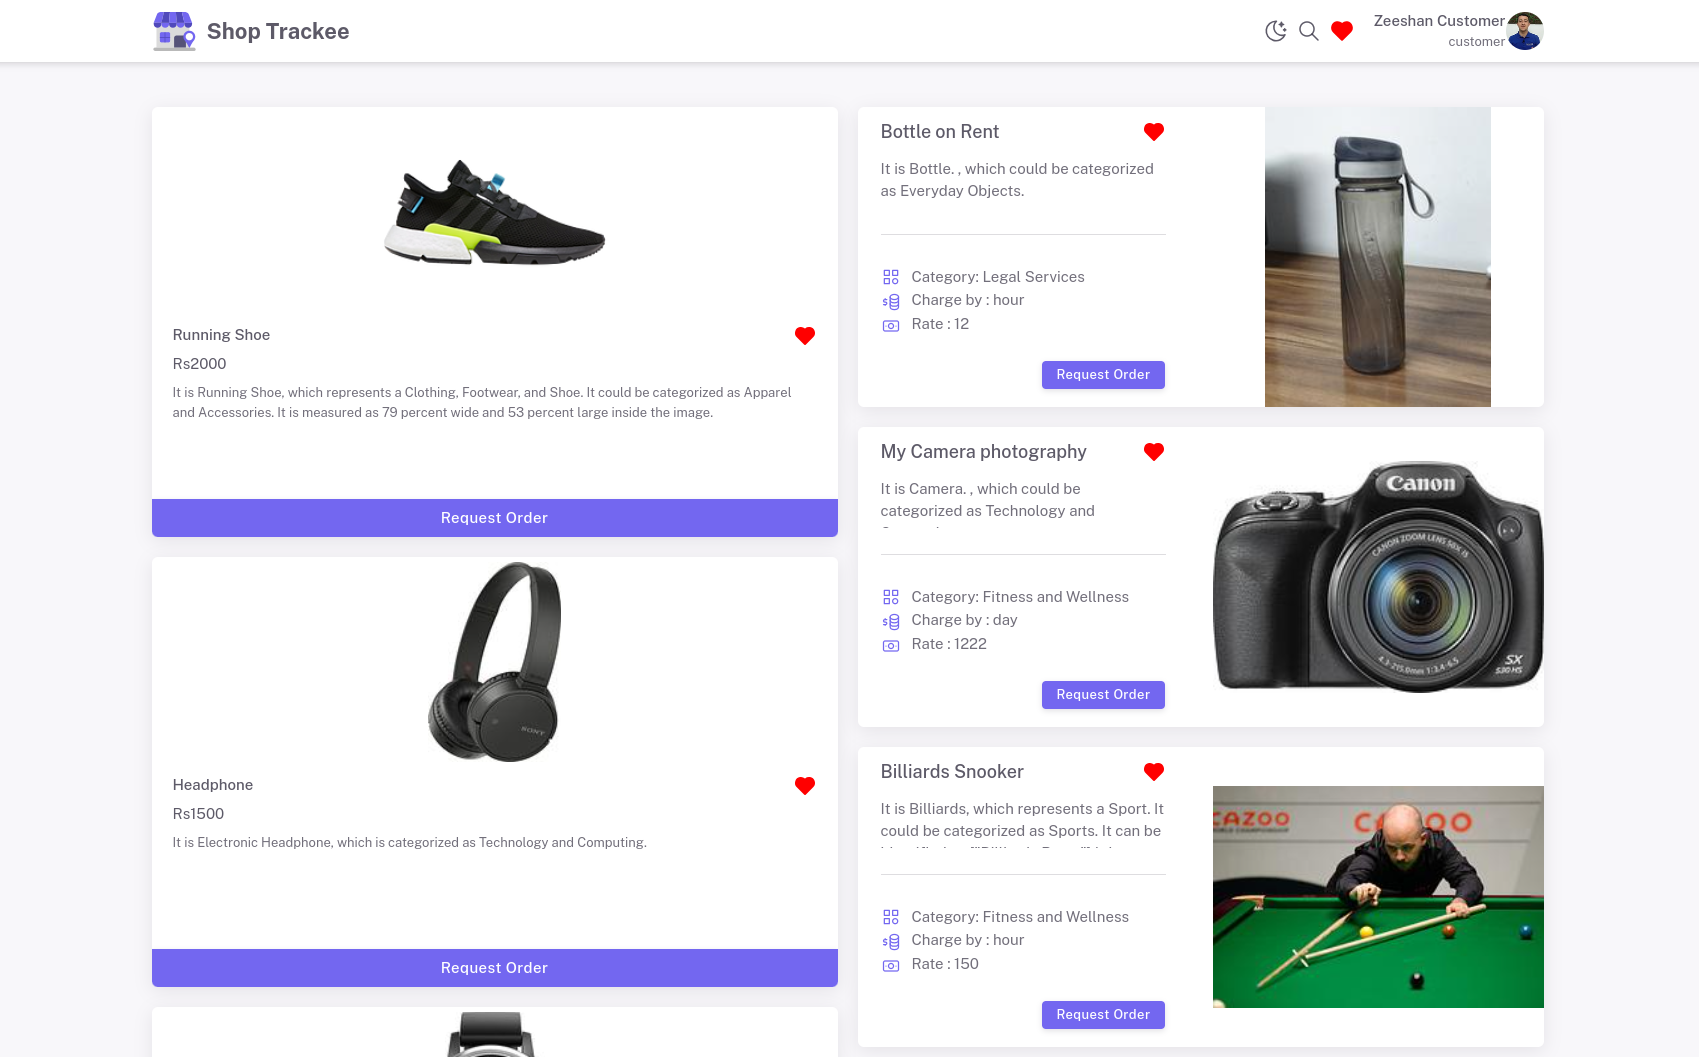
\includegraphics[width=1\textwidth]{customer-all-favorites-page}
	\caption{Track My Shop - Customer Favorites}
\end{figure}


\begin{figure}[h]
	\subsection{Dark Mode }
	\centering
	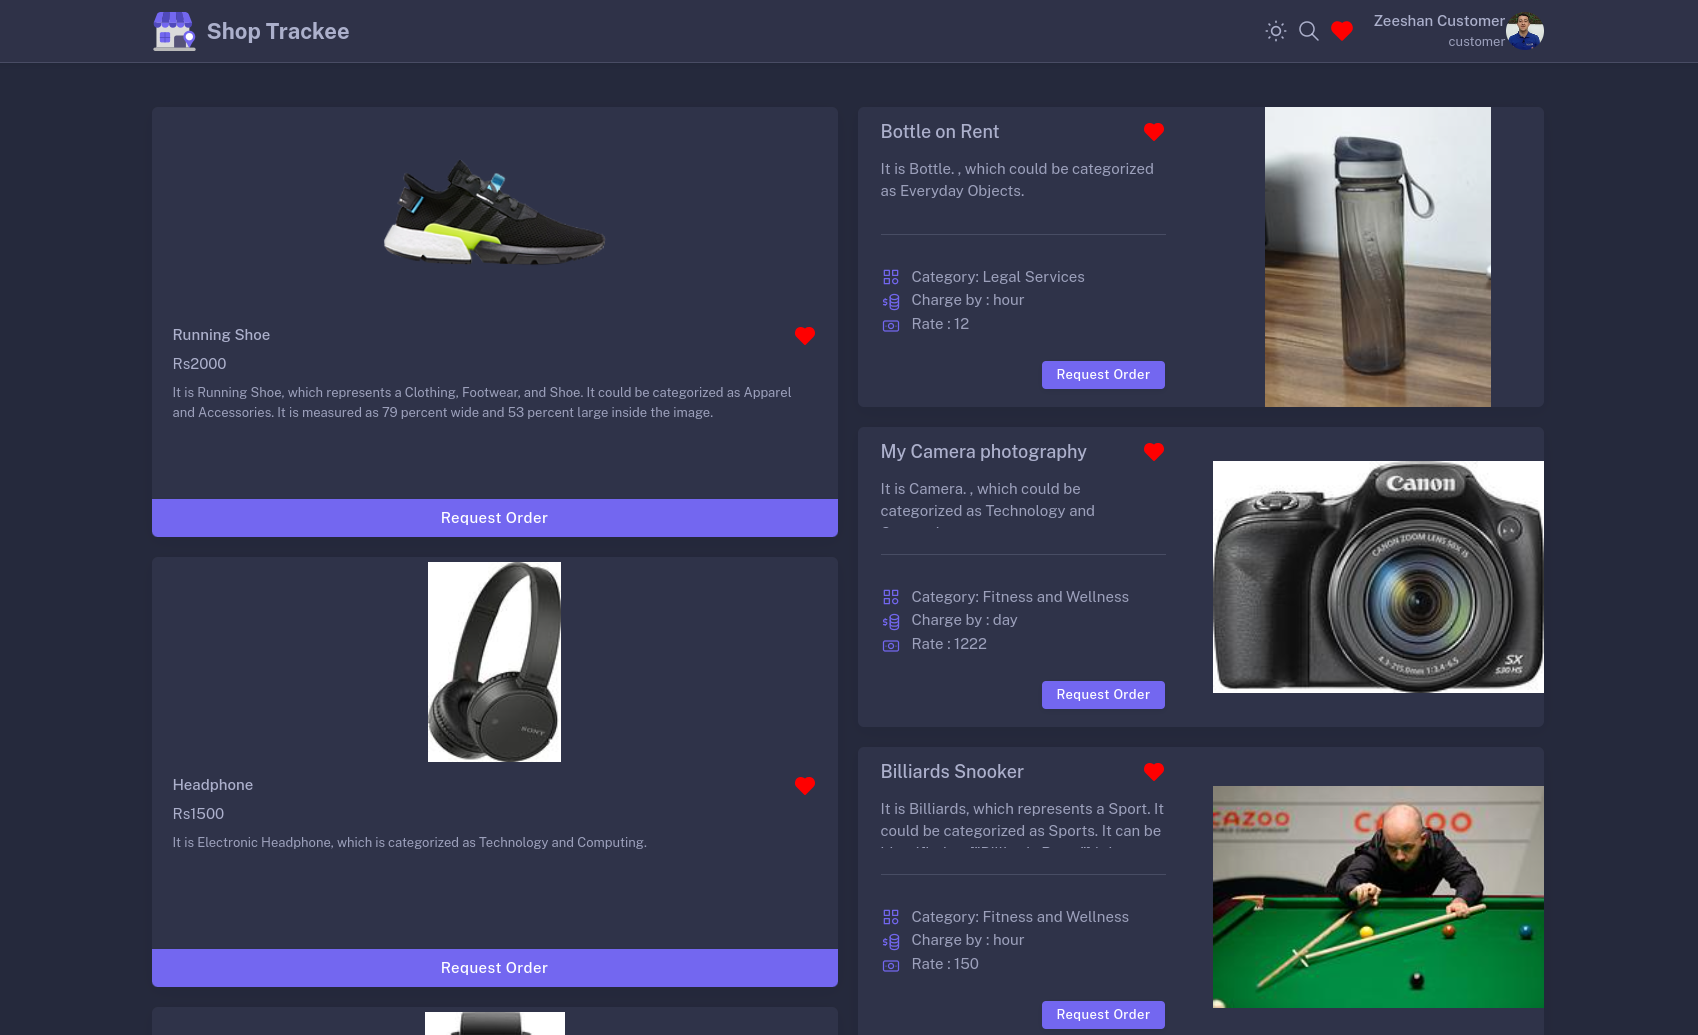
\includegraphics[width=0.9\textwidth]{dark-mode-favorites-page}
	\caption{Track My Shop - Dark Mode}
\end{figure}

\pagebreak
\section{Hardware Interface}
The "Track My Shop" web application is primarily a software-based system that relies on internet connectivity and web browsers to function. However, there are a few essential hardware components and interfaces that enable its operation:

\begin{itemize}
	\item Computer Systems (Desktops, Laptops, Tablets)
	\item Smartphones and Mobile Devices
	\item Stable Internet Connection
	\item Cameras (for Image Capture)
	\item Global Positioning System (GPS) and Location Services
	\item Input Devices (Keyboards, Mouse, Touchscreens)
\end{itemize}

\subsection{Hardware Requirements}
Here are some minimal requirements of hardware to run this Web Application:
\begin{itemize}
	\item Processor: core i5 - 2.0GHz  
	\item RAM 4 GB+ 
	\item Free System Storage (minimum 2 GB)
	\item Operating System: Windows, Linux, Mac, Andriod, IOS
	\item Browsers (Chrome 64+, Edge 79+, Firefox 67+, Opera 51+, Safari 12+)
	\item GPS WGS 84 (World Geodetic System 1984) datum for Google Maps 
\end{itemize}


\section{Evaluation}
Each element of our website is meticulously designed based on the findings of Market Shop Sellers and Customer Research, which takes into account criteria such as technical knowledge, and comprehension.The user is given a seamless experience, allowing them to easily see, update, upload, and manage their data. While designing the website, Human Computer Interaction concepts were taken into account, allowing the user to see where they are presently working and easy to use. Before releasing the website, we make sure that all of the tabs and buttons are visible and double-checked and everything is working properly. Once the website is ready for the user, it will be extensively tested and any necessary changes will be done. Hence the website is user friendly and unambiguous.

\section{Unit Testing}

Unit testing is a crucial component of the development process in "Track My Shop." It involves testing individual units or components of the application to ensure their accuracy, reliability, and correctness. The primary focus is to verify that each unit of the software performs as designed.

In this project, unit testing will encompass the following aspects:

\subsection{Frontend Components} Test individual frontend components like UI elements, input fields, buttons, and their respective functionalities to ensure proper rendering and interactivity.
	
\subsection{Backend API Endpoints} Test the backend API endpoints using testing frameworks to verify their response, data integrity, error handling, and authentication mechanisms.
	
\subsection{Database Interactions} Test the interactions with the database, including CRUD operations, to ensure accurate data retrieval, storage, and manipulation.
	
\subsection{Integration Testing} Conduct integration tests to validate the interaction and communication between different modules, ensuring the overall system functions seamlessly.
	
\subsection{Error Handling and Edge Cases} Perform tests to evaluate the system's behavior under various error conditions and edge cases to guarantee robustness and graceful error handling.


Adopting a comprehensive unit testing strategy will enhance the project's quality, reduce bugs, and provide a stable and reliable application for users.

\section{Test Cases}
Unit testing is a crucial component of the development process in "Track My Shop". It involves testing individual units or components of the application to ensure their accuracy, reliability, and correctness. The primary focus is to verify that each unit of the software performs as designed. Here are some test cases for major units of the application:

\pagebreak

\subsection{Frontend Components}
Here are the unit test cases for the frontend components:	

\textbf{\\}
\textbf{\\}


% Table for User Registration Form Validation test case
\begin{table}[h]
	\subsubsection{Test Case 1: User Registration Form Validation}
	\centering
	\caption{User Registration Form Validation (TC1)}
	\begin{tabular}{|p{0.3\linewidth}|p{0.6\linewidth}|}
		\hline
		\textbf{Test Case ID} & TC1 \\
		\hline
		\textbf{Test Case Name} & User Registration Form Validation \\
		\hline
		\textbf{Component} & User Registration Form \\
		\hline
		\textbf{Input} & Incomplete or incorrect user registration details \\
		\hline
		\textbf{Expected Output} & Prevent registration and display appropriate validation errors \\
		\hline
		\textbf{Test Steps} & 
		\begin{enumerate}
			\item Fill the registration form with incomplete or incorrect details
			\item Attempt to submit the registration form
			\item Check the interface to verify appropriate validation errors are displayed
		\end{enumerate} \\
		\hline
		\textbf{Execution Result} & Pass \\
		\hline
	\end{tabular}
\end{table}


\newpage
% Table for Product Image Uploading test case
\begin{table}[h]
	\subsubsection{Test Case 2: Product/Service Image Uploading \& Recognition}
	\centering
	\caption{Product Image Uploading (TC2)}
	\begin{tabular}{|p{0.3\linewidth}|p{0.6\linewidth}|}
		\hline
		\textbf{Test Case ID} & TC2 \\
		\hline
		\textbf{Test Case Name} & Product/Service Image Uploading and Recognition \\
		\hline
		\textbf{Component} & Product/Service Image Chooser / Image Capturing Camera\\
		\hline
		\textbf{Input} & Image upload/capture request \\
		\hline
		\textbf{Expected Output} & Successful image upload and display in the product/service management UI \\
		\hline
		\textbf{Test Steps} & 
		\begin{enumerate}
			\item Initiate image upload process
			\item Check the Recognize Image button visibility under image
			\item Recognize Image by using button
			\item Check the UI to verify the image is displayed appropriately
			\item Check the product/service form to verify recognized data
		\end{enumerate} \\
		\hline
		\textbf{Execution Result} & Pass \\
		\hline
	\end{tabular}
\end{table}
\pagebreak

\begin{table}[h]
	\subsubsection{Test Case 3: Product/Service Component Rendering}
	\centering
	\caption{Unit Test for Rendering Product/Service Display Component (TC3)}
	\begin{tabular}{|p{0.3\linewidth}|p{0.6\linewidth}|}
		\hline
		\textbf{Test Case ID} & TC3 \\
		\hline
		\textbf{Test Case Name} & Rendering Product/Service Display \\
		\hline
		\textbf{Component} & Product/Service Display Component \\
		\hline
		\textbf{Input} & None (Component rendering) \\
		\hline
		\textbf{Expected Output} & Rendered product/service display \\
		\hline
		\textbf{Test Steps} & \begin{enumerate}
			\item Load the application 
			\item Navigate to the page where the products/services display component is rendered 
		\end{enumerate} \\
		\hline
		\textbf{Execution Result} & Pass \\
		\hline
	\end{tabular}
\end{table}




% Table for Order Request with Message test case
\begin{table}[h]
	\subsubsection{Test Case 4: Order Request with Message}
	\centering
	\caption{Order Request with Message (TC4)}
	\begin{tabular}{|p{0.3\linewidth}|p{0.6\linewidth}|}
		\hline
		\textbf{Test Case ID} & TC4 \\
		\hline
		\textbf{Test Case Name} & Order Request with Message \\
		\hline
		\textbf{Component} & Order Management UI \\
		\hline
		\textbf{Input} & Order request along with an optional message from the customer \\
		\hline
		\textbf{Expected Output} & Successful submission of the order request with the attached message \\
		\hline
		\textbf{Test Steps} & 
		\begin{enumerate}
			\item Select a product and initiate the order request process
			\item Provide additional instructions or messages (optional)
			\item Complete the order request
			\item Check all order requests table to verify the order request was successful
		\end{enumerate} \\
		\hline
		\textbf{Execution Result} & Pass \\
		\hline
	\end{tabular}
\end{table}

\pagebreak
% Table for Search Bar Functionality test case
\begin{table}[h]
	\subsubsection{Test Case 5: Search Box Functionality}
	\centering
	\caption{Search Bar Functionality (TC5)}
	\begin{tabular}{|p{0.3\linewidth}|p{0.6\linewidth}|}
		\hline
		\textbf{Test Case ID} & TC5 \\
		\hline
		\textbf{Test Case Name} & Search Box Functionality \\
		\hline
		\textbf{Component} & Search Bar, Image Capturing Camera, Search Radius Field \\
		\hline
		\textbf{Input} & Search query, Search Image, Distance radius \\
		\hline
		\textbf{Expected Output} & Display of relevant search results \\
		\hline
		\textbf{Test Steps} & 
		\begin{enumerate}
			\item Enter a search query in the search bar
			\item Initiate the search process
			\item Check the interface to verify relevant search results are displayed
		\end{enumerate} \\
		\hline
		\textbf{Execution Result} & Pass \\
		\hline
	\end{tabular}
\end{table}


\subsection{Backend API Endpoints}

Here are the unit test cases for the backend API endpoints:

\begin{table}[h]
	\subsubsection{Test Case 6: Response of Product Listing Endpoint}
	\centering
	\caption{Test Case for Response of Product Listing Endpoint (TC6)}
	\begin{tabular}{|p{0.3\linewidth}|p{0.6\linewidth}|}
		\hline
		\textbf{Test Case ID} & TC6 \\
		\hline
		\textbf{Test Case Name} & Response of Product Listing Endpoint \\
		\hline
		\textbf{Endpoint} & Product Listing \\
		\hline
		\textbf{Input} & Send a request to the product listing endpoint \\
		\hline
		\textbf{Expected Output} & Receive a list of products \\
		\hline
		\textbf{Test Steps} & \begin{enumerate}
			\item Send a valid request to the product listing endpoint 
			\item Receive the response from the endpoint 
		\end{enumerate}\\
		\hline
		\textbf{Execution Result} & Pass \\
		\hline
	\end{tabular}
\end{table}


\begin{table}[h]
	\subsubsection{Test Case 7: Error Handling of Invalid Request}
	\centering
	\caption{Test Case for Error Handling of Invalid Request (TC7)}
	\begin{tabular}{|p{0.3\linewidth}|p{0.6\linewidth}|}
		\hline
		\textbf{Test Case ID} & TC7 \\
		\hline
		\textbf{Test Case Name} & Error Handling of Invalid Request \\
		\hline
		\textbf{Endpoint} & Any API Endpoint \\
		\hline
		\textbf{Input} & Send an invalid request \\
		\hline
		\textbf{Expected Output} & Receive an appropriate error response \\
		\hline
		\textbf{Test Steps} & \begin{enumerate}
			\item Send an invalid request to the specified endpoint
			\item Receive the error response from the endpoint
		\end{enumerate} \\
		\hline
		\textbf{Execution Result} & Pass \\
		\hline
	\end{tabular}
\end{table}


\pagebreak
\subsection{Database Interactions}

% Table for Product Data Retrieval test case
\begin{table}[h]
	\subsubsection{Test Case 8: Product Data Retrieval}
	\centering
	\caption{Product Data Retrieval (TC8)}
	\begin{tabular}{|p{0.3\linewidth}|p{0.6\linewidth}|}
		\hline
		\textbf{Test Case ID} & TC8 \\
		\hline
		\textbf{Test Case Name} & Product Data Retrieval \\
		\hline
		\textbf{Component} & Database Interaction \\
		\hline
		\textbf{Input} & Request to retrieve product data \\
		\hline
		\textbf{Expected Output} & Valid product data from the database \\
		\hline
		\textbf{Test Steps} & \begin{enumerate}
			\item Send a request to retrieve product data	
			\item Check the received product data
		\end{enumerate}\\
		\hline
		\textbf{Execution Result} & Pass \\
		\hline
	\end{tabular}
\end{table}


% Table for Adding New Product test case
\begin{table}[h]
	\subsubsection{Test Case 9: Adding New Product}
	\centering
	\caption{Adding New Product (TC9)}
	\begin{tabular}{|p{0.3\linewidth}|p{0.6\linewidth}|}
		\hline
		\textbf{Test Case ID} & TC9 \\
		\hline
		\textbf{Test Case Name} & Adding New Product \\
		\hline
		\textbf{Component} & Database Interaction \\
		\hline
		\textbf{Input} & New product details (name, description, price, etc.) \\
		\hline
		\textbf{Expected Output} & Product added successfully in the database \\
		\hline
		\textbf{Test Steps} & \begin{enumerate}
			\item Provide input for a new product 
			\item Initiate the process to add the product
			\item Check the response to verify successful addition
			\end{enumerate} \\
		\hline
		\textbf{Execution Result} & Pass \\
		\hline
	\end{tabular}
\end{table}

\pagebreak
\subsection{Integration Testing}

% Table for Integration of User Authentication test case
\begin{table}[h]
	\subsubsection{Test Case 10: Integration of User Authentication}
	\centering
	\caption{Integration of User Authentication (TC10)}
	\begin{tabular}{|p{0.3\linewidth}|p{0.6\linewidth}|}
		\hline
		\textbf{Test Case ID} & TC10 \\
		\hline
		\textbf{Test Case Name} & Integration of User Authentication \\
		\hline
		\textbf{Components} & Authentication Module, Database Interaction \\
		\hline
		\textbf{Input} & User credentials \\
		\hline
		\textbf{Expected Output} & Successful user authentication \\
		\hline
		\textbf{Test Steps} & 
		\begin{enumerate}
			\item Provide user credentials
			\item Initiate the authentication process
			\item Check the response to verify successful authentication
		\end{enumerate} \\
		\hline
		\textbf{Execution Result} & Pass \\
		\hline
	\end{tabular}
\end{table}

% Table for Integration of Product Listing test case
\begin{table}[h]
	\subsubsection{Test Case 11: Integration of Product Listing}
	\centering
	\caption{Integration of Product Listing (TC11)}
	\begin{tabular}{|p{0.3\linewidth}|p{0.6\linewidth}|}
		\hline
		\textbf{Test Case ID} & TC11 \\
		\hline
		\textbf{Test Case Name} & Integration of Product Listing \\
		\hline
		\textbf{Components} & Product Listing Module, Database Interaction \\
		\hline
		\textbf{Input} & Request to list products \\
		\hline
		\textbf{Expected Output} & Successful retrieval of product listing \\
		\hline
		\textbf{Test Steps} & 
		\begin{enumerate}
			\item Send a request to list products
			\item Check the response to verify the successful retrieval of product listing
		\end{enumerate} \\
		\hline
		\textbf{Execution Result} & Pass \\
		\hline
	\end{tabular}
\end{table}

\pagebreak
\subsection{Error Handling and Edge Cases}


% Table for Invalid User Authentication test case
\begin{table}[h]
	\subsubsection{Test Case 12: Invalid User Authentication}
	\centering
	\caption{Invalid User Authentication (TC12)}
	\begin{tabular}{|p{0.3\linewidth}|p{0.6\linewidth}|}
		\hline
		\textbf{Test Case ID} & TC12 \\
		\hline
		\textbf{Test Case Name} & Invalid User Authentication \\
		\hline
		\textbf{Components} & Authentication Module, Database Interaction \\
		\hline
		\textbf{Input} & Incorrect user credentials \\
		\hline
		\textbf{Expected Output} & Authentication failure with appropriate error message \\
		\hline
		\textbf{Test Steps} & 
		\begin{enumerate}
			\item Provide incorrect user credentials
			\item Initiate the authentication process
			\item Check the response to verify authentication failure and error message
		\end{enumerate} \\
		\hline
		\textbf{Execution Result} & Pass \\
		\hline
	\end{tabular}
\end{table}

% Table for Product Listing Empty test case
\begin{table}[h]
	\subsubsection{Test Case 13: Product Listing Empty}
	\centering
	\caption{Product Listing Empty (TC13)}
	\begin{tabular}{|p{0.3\linewidth}|p{0.6\linewidth}|}
		\hline
		\textbf{Test Case ID} & TC13 \\
		\hline
		\textbf{Test Case Name} & Product Listing Empty \\
		\hline
		\textbf{Components} & Product Listing Module, Database Interaction \\
		\hline
		\textbf{Input} & Request to list products when no products are available \\
		\hline
		\textbf{Expected Output} & Successful retrieval with an empty product list \\
		\hline
		\textbf{Test Steps} & 
		\begin{enumerate}
			\item Send a request to list products
			\item Check the response to verify an empty product list
		\end{enumerate} \\
		\hline
		\textbf{Execution Result} & Pass \\
		\hline
	\end{tabular}
\end{table}

% Add more test cases for Error Handling and Edge Cases as needed
%-----------------------
\pagebreak

% Table for Invalid Product Addition test case
\begin{table}[h]
	\subsubsection{Test Case 14: Invalid Product Addition}
	\centering
	\caption{Invalid Product Addition (TC14)}
	\begin{tabular}{|p{0.3\linewidth}|p{0.6\linewidth}|}
		\hline
		\textbf{Test Case ID} & TC14 \\
		\hline
		\textbf{Test Case Name} & Invalid Product Addition \\
		\hline
		\textbf{Components} & Product Management Module, Database Interaction \\
		\hline
		\textbf{Input} & Incomplete or incorrect product details \\
		\hline
		\textbf{Expected Output} & Failure to add the product with an appropriate error message \\
		\hline
		\textbf{Test Steps} & 
		\begin{enumerate}
			\item Provide incomplete or incorrect product details
			\item Attempt to add the product
			\item Check the response to verify the error message
		\end{enumerate} \\
		\hline
		\textbf{Execution Result} & Pass \\
		\hline
	\end{tabular}
\end{table}



%---------------------------------


\pagebreak
\section{Functional Testing}

Functional testing is a critical aspect of ensuring the "Track My Shop" application meets its intended functional requirements. This type of testing involves validating the software's functions and features against the specified requirements and design. It primarily focuses on what the system does.

Functional testing for this project encompasses the following areas:

\subsection{User Authentication and Authorization} Validate the authentication process to ensure users can securely create accounts, log in, and access appropriate functionalities based on their roles.

\subsection{Product and Service Listings} Verify that sellers can effectively list their products and services using various methods, including image recognition and manual entry, and customers can view and search these listings.

\subsection{Order Placement and Management} Test the ordering process to ensure customers can place orders for products and services, sellers receive order requests, and they can manage and respond to these orders appropriately.

\subsection{Location-Based Features} Validate the location-based functionalities such as finding nearby shops, setting a search radius, and accessing directions to physical shops.

\subsection{Search and Filtering} Verify the accuracy and efficiency of the search and filtering capabilities, allowing users to search for products, services, or shops based on various criteria.

\subsection{Error Handling} Test the system's behavior under erroneous conditions, ensuring that appropriate error messages and notifications are displayed to users.

\subsection{UI/UX Testing} Evaluate the user interface and overall user experience to ensure it is intuitive, consistent, and adheres to design guidelines.
	

Functional testing ensures that the "Track My Shop" application performs its intended functions correctly, providing users with a seamless and reliable experience.


\subsection{Testing Requirements}

Functional testing for this web application necessitates a comprehensive approach that covers various functionalities and ensures their correctness and reliability. The testing requirements include:

\subsubsection{User Authentication:}
	\begin{itemize}
		\item Verify that users can create accounts securely with the necessary role and personal information.
		\item Test login functionality, ensuring users can authenticate themselves with correct credentials.
		\item Validate the behavior of the system in case of incorrect login attempts, including appropriate error messages.
	\end{itemize}
	
\subsubsection{Product and Service Listings:}
	\begin{itemize}
		\item Ensure sellers can accurately list products and services using various methods like image recognition, capturing image, and choosing image manually or manual entry.
		\item Validate that sellers can edit, delete, and update product and service information as needed.
		\item Verify that customers can view and filter product and service listings with ease.
	\end{itemize}
	
\subsubsection{Orders Management:}
	\begin{itemize}
		\item Test the process of requesting orders, ensuring customers can successfully initiate orders for desired products and services.
		\item Validate that sellers receive order requests promptly and can manage them effectively, including accepting or rejecting order requests.
		\item Verify that customers receive timely notifications and updates on their orders.
	\end{itemize}
	
\subsubsection{Location-Based Features:}
	\begin{itemize}
		\item Ensure users can find nearby shops based on their location and specified search radius.
		\item Validate the accuracy of location-based search results, providing users with relevant and nearby options.
		\item Test the functionality of accessing directions to physical shops from the user's current location.
	\end{itemize}
	
\subsubsection{Search and Filtering:}
	\begin{itemize}
		\item Validate the accuracy and efficiency of the search feature, allowing users to search for products, services, or shops based on keywords.
		\item Test capabilities to ensure users can search based on image, categories, or other relevant criteria.
	\end{itemize}
	
\subsubsection{Error Handling:}
	\begin{itemize}
		\item Verify that the system displays appropriate error messages and notifications for incorrect inputs or erroneous actions.
		\item Test the behavior of the system under unexpected conditions, ensuring graceful handling of errors to prevent system crashes.
	\end{itemize}
	
\subsubsection{UI/UX Testing:}
	\begin{itemize}
		\item Validate that the user interface is consistent, intuitive, and adheres to design guidelines.
		\item Test the responsiveness of the application across various devices and screen sizes.
	\end{itemize}

These testing requirements form the basis for comprehensive functional testing, ensuring the application meets its intended functionalities reliably and accurately.











